%% bare_conf.tex
%% V1.4
%% 2012/12/27
%% by Michael Shell
%% See:
%% http://www.michaelshell.org/
%% for current contact information.
%%
%% This is a skeleton file demonstrating the use of IEEEtran.cls
%% (requires IEEEtran.cls version 1.8 or later) with an IEEE conference paper.
%%
%% Support sites:
%% http://www.michaelshell.org/tex/ieeetran/
%% http://www.ctan.org/tex-archive/macros/latex/contrib/IEEEtran/
%% and
%% http://www.ieee.org/

%%*************************************************************************
%% Legal Notice:
%% This code is offered as-is without any warranty either expressed or
%% implied; without even the implied warranty of MERCHANTABILITY or
%% FITNESS FOR A PARTICULAR PURPOSE! 
%% User assumes all risk.
%% In no event shall IEEE or any contributor to this code be liable for
%% any damages or losses, including, but not limited to, incidental,
%% consequential, or any other damages, resulting from the use or misuse
%% of any information contained here.
%%
%% All comments are the opinions of their respective authors and are not
%% necessarily endorsed by the IEEE.
%%
%% This work is distributed under the LaTeX Project Public License (LPPL)
%% ( http://www.latex-project.org/ ) version 1.3, and may be freely used,
%% distributed and modified. A copy of the LPPL, version 1.3, is included
%% in the base LaTeX documentation of all distributions of LaTeX released
%% 2003/12/01 or later.
%% Retain all contribution notices and credits.
%% ** Modified files should be clearly indicated as such, including  **
%% ** renaming them and changing author support contact information. **
%%
%% File list of work: IEEEtran.cls, IEEEtran_HOWTO.pdf, bare_adv.tex,
%%                    bare_conf.tex, bare_jrnl.tex, bare_jrnl_compsoc.tex,
%%                    bare_jrnl_transmag.tex
%%*************************************************************************

% *** Authors should verify (and, if needed, correct) their LaTeX system  ***
% *** with the testflow diagnostic prior to trusting their LaTeX platform ***
% *** with production work. IEEE's font choices can trigger bugs that do  ***
% *** not appear when using other class files.                            ***
% The testflow support page is at:
% http://www.michaelshell.org/tex/testflow/



% Note that the a4paper option is mainly intended so that authors in
% countries using A4 can easily print to A4 and see how their papers will
% look in print - the typesetting of the document will not typically be
% affected with changes in paper size (but the bottom and side margins will).
% Use the testflow package mentioned above to verify correct handling of
% both paper sizes by the user's LaTeX system.
%
% Also note that the "draftcls" or "draftclsnofoot", not "draft", option
% should be used if it is desired that the figures are to be displayed in
% draft mode.
%
\documentclass[conference]{IEEEtran}
% Add the compsoc option for Computer Society conferences.
%
% If IEEEtran.cls has not been installed into the LaTeX system files,
% manually specify the path to it like:
% \documentclass[conference]{../sty/IEEEtran}





% Some very useful LaTeX packages include:
% (uncomment the ones you want to load)


% *** MISC UTILITY PACKAGES ***
%
%\usepackage{ifpdf}
% Heiko Oberdiek's ifpdf.sty is very useful if you need conditional
% compilation based on whether the output is pdf or dvi.
% usage:
% \ifpdf
%   % pdf code
% \else
%   % dvi code
% \fi
% The latest version of ifpdf.sty can be obtained from:
% http://www.ctan.org/tex-archive/macros/latex/contrib/oberdiek/
% Also, note that IEEEtran.cls V1.7 and later provides a builtin
% \ifCLASSINFOpdf conditional that works the same way.
% When switching from latex to pdflatex and vice-versa, the compiler may
% have to be run twice to clear warning/error messages.






% *** CITATION PACKAGES ***
%
%\usepackage{cite}
% cite.sty was written by Donald Arseneau
% V1.6 and later of IEEEtran pre-defines the format of the cite.sty package
% \cite{} output to follow that of IEEE. Loading the cite package will
% result in citation numbers being automatically sorted and properly
% "compressed/ranged". e.g., [1], [9], [2], [7], [5], [6] without using
% cite.sty will become [1], [2], [5]--[7], [9] using cite.sty. cite.sty's
% \cite will automatically add leading space, if needed. Use cite.sty's
% noadjust option (cite.sty V3.8 and later) if you want to turn this off
% such as if a citation ever needs to be enclosed in parenthesis.
% cite.sty is already installed on most LaTeX systems. Be sure and use
% version 4.0 (2003-05-27) and later if using hyperref.sty. cite.sty does
% not currently provide for hyperlinked citations.
% The latest version can be obtained at:
% http://www.ctan.org/tex-archive/macros/latex/contrib/cite/
% The documentation is contained in the cite.sty file itself.






% *** GRAPHICS RELATED PACKAGES ***
%
\ifCLASSINFOpdf
  % \usepackage[pdftex]{graphicx}
  % declare the path(s) where your graphic files are
  % \graphicspath{{../pdf/}{../jpeg/}}
  % and their extensions so you won't have to specify these with
  % every instance of \includegraphics
  % \DeclareGraphicsExtensions{.pdf,.jpeg,.png}
\else
  % or other class option (dvipsone, dvipdf, if not using dvips). graphicx
  % will default to the driver specified in the system graphics.cfg if no
  % driver is specified.
  % \usepackage[dvips]{graphicx}
  % declare the path(s) where your graphic files are
  % \graphicspath{{../eps/}}
  % and their extensions so you won't have to specify these with
  % every instance of \includegraphics
  % \DeclareGraphicsExtensions{.eps}
\fi
% graphicx was written by David Carlisle and Sebastian Rahtz. It is
% required if you want graphics, photos, etc. graphicx.sty is already
% installed on most LaTeX systems. The latest version and documentation
% can be obtained at: 
% http://www.ctan.org/tex-archive/macros/latex/required/graphics/
% Another good source of documentation is "Using Imported Graphics in
% LaTeX2e" by Keith Reckdahl which can be found at:
% http://www.ctan.org/tex-archive/info/epslatex/
%
% latex, and pdflatex in dvi mode, support graphics in encapsulated
% postscript (.eps) format. pdflatex in pdf mode supports graphics
% in .pdf, .jpeg, .png and .mps (metapost) formats. Users should ensure
% that all non-photo figures use a vector format (.eps, .pdf, .mps) and
% not a bitmapped formats (.jpeg, .png). IEEE frowns on bitmapped formats
% which can result in "jaggedy"/blurry rendering of lines and letters as
% well as large increases in file sizes.
%
% You can find documentation about the pdfTeX application at:
% http://www.tug.org/applications/pdftex





% *** MATH PACKAGES ***
%
\usepackage[cmex10]{amsmath}
% A popular package from the American Mathematical Society that provides
% many useful and powerful commands for dealing with mathematics. If using
% it, be sure to load this package with the cmex10 option to ensure that
% only type 1 fonts will utilized at all point sizes. Without this option,
% it is possible that some math symbols, particularly those within
% footnotes, will be rendered in bitmap form which will result in a
% document that can not be IEEE Xplore compliant!
%
% Also, note that the amsmath package sets \interdisplaylinepenalty to 10000
% thus preventing page breaks from occurring within multiline equations. Use:
%\interdisplaylinepenalty=2500
% after loading amsmath to restore such page breaks as IEEEtran.cls normally
% does. amsmath.sty is already installed on most LaTeX systems. The latest
% version and documentation can be obtained at:
% http://www.ctan.org/tex-archive/macros/latex/required/amslatex/math/





% *** SPECIALIZED LIST PACKAGES ***
%
%\usepackage{algorithmic}
% algorithmic.sty was written by Peter Williams and Rogerio Brito.
% This package provides an algorithmic environment fo describing algorithms.
% You can use the algorithmic environment in-text or within a figure
% environment to provide for a floating algorithm. Do NOT use the algorithm
% floating environment provided by algorithm.sty (by the same authors) or
% algorithm2e.sty (by Christophe Fiorio) as IEEE does not use dedicated
% algorithm float types and packages that provide these will not provide
% correct IEEE style captions. The latest version and documentation of
% algorithmic.sty can be obtained at:
% http://www.ctan.org/tex-archive/macros/latex/contrib/algorithms/
% There is also a support site at:
% http://algorithms.berlios.de/index.html
% Also of interest may be the (relatively newer and more customizable)
% algorithmicx.sty package by Szasz Janos:
% http://www.ctan.org/tex-archive/macros/latex/contrib/algorithmicx/




% *** ALIGNMENT PACKAGES ***
%
%\usepackage{array}
% Frank Mittelbach's and David Carlisle's array.sty patches and improves
% the standard LaTeX2e array and tabular environments to provide better
% appearance and additional user controls. As the default LaTeX2e table
% generation code is lacking to the point of almost being broken with
% respect to the quality of the end results, all users are strongly
% advised to use an enhanced (at the very least that provided by array.sty)
% set of table tools. array.sty is already installed on most systems. The
% latest version and documentation can be obtained at:
% http://www.ctan.org/tex-archive/macros/latex/required/tools/


% IEEEtran contains the IEEEeqnarray family of commands that can be used to
% generate multiline equations as well as matrices, tables, etc., of high
% quality.




% *** SUBFIGURE PACKAGES ***
%\ifCLASSOPTIONcompsoc
%  \usepackage[caption=false,font=normalsize,labelfont=sf,textfont=sf]{subfig}
%\else
%  \usepackage[caption=false,font=footnotesize]{subfig}
%\fi
% subfig.sty, written by Steven Douglas Cochran, is the modern replacement
% for subfigure.sty, the latter of which is no longer maintained and is
% incompatible with some LaTeX packages including fixltx2e. However,
% subfig.sty requires and automatically loads Axel Sommerfeldt's caption.sty
% which will override IEEEtran.cls' handling of captions and this will result
% in non-IEEE style figure/table captions. To prevent this problem, be sure
% and invoke subfig.sty's "caption=false" package option (available since
% subfig.sty version 1.3, 2005/06/28) as this is will preserve IEEEtran.cls
% handling of captions.
% Note that the Computer Society format requires a larger sans serif font
% than the serif footnote size font used in traditional IEEE formatting
% and thus the need to invoke different subfig.sty package options depending
% on whether compsoc mode has been enabled.
%
% The latest version and documentation of subfig.sty can be obtained at:
% http://www.ctan.org/tex-archive/macros/latex/contrib/subfig/




% *** FLOAT PACKAGES ***
%
%\usepackage{fixltx2e}
% fixltx2e, the successor to the earlier fix2col.sty, was written by
% Frank Mittelbach and David Carlisle. This package corrects a few problems
% in the LaTeX2e kernel, the most notable of which is that in current
% LaTeX2e releases, the ordering of single and double column floats is not
% guaranteed to be preserved. Thus, an unpatched LaTeX2e can allow a
% single column figure to be placed prior to an earlier double column
% figure. The latest version and documentation can be found at:
% http://www.ctan.org/tex-archive/macros/latex/base/


%\usepackage{stfloats}
% stfloats.sty was written by Sigitas Tolusis. This package gives LaTeX2e
% the ability to do double column floats at the bottom of the page as well
% as the top. (e.g., "\begin{figure*}[!b]" is not normally possible in
% LaTeX2e). It also provides a command:
%\fnbelowfloat
% to enable the placement of footnotes below bottom floats (the standard
% LaTeX2e kernel puts them above bottom floats). This is an invasive package
% which rewrites many portions of the LaTeX2e float routines. It may not work
% with other packages that modify the LaTeX2e float routines. The latest
% version and documentation can be obtained at:
% http://www.ctan.org/tex-archive/macros/latex/contrib/sttools/
% Do not use the stfloats baselinefloat ability as IEEE does not allow
% \baselineskip to stretch. Authors submitting work to the IEEE should note
% that IEEE rarely uses double column equations and that authors should try
% to avoid such use. Do not be tempted to use the cuted.sty or midfloat.sty
% packages (also by Sigitas Tolusis) as IEEE does not format its papers in
% such ways.
% Do not attempt to use stfloats with fixltx2e as they are incompatible.
% Instead, use Morten Hogholm'a dblfloatfix which combines the features
% of both fixltx2e and stfloats:
%
% \usepackage{dblfloatfix}
% The latest version can be found at:
% http://www.ctan.org/tex-archive/macros/latex/contrib/dblfloatfix/




% *** PDF, URL AND HYPERLINK PACKAGES ***
%
%\usepackage{url}
% url.sty was written by Donald Arseneau. It provides better support for
% handling and breaking URLs. url.sty is already installed on most LaTeX
% systems. The latest version and documentation can be obtained at:
% http://www.ctan.org/tex-archive/macros/latex/contrib/url/
% Basically, \url{my_url_here}.




% *** Do not adjust lengths that control margins, column widths, etc. ***
% *** Do not use packages that alter fonts (such as pslatex).         ***
% There should be no need to do such things with IEEEtran.cls V1.6 and later.
% (Unless specifically asked to do so by the journal or conference you plan
% to submit to, of course. )


% correct bad hyphenation here
\hyphenation{op-tical net-works semi-conduc-tor}

\usepackage{graphicx}
\usepackage{acronym}
\usepackage{xspace}


\begin{document}


%
% paper title
% can use linebreaks \\ within to get better formatting as desired
% Do not put math or special symbols in the title.
\title{Preliminary Results in ADCP-aided Navigation for Autonomous Underwater Gliders}
%
% author names and affiliations
% use a multiple column layout for up to three different
% affiliations
%\author{
%Michael V. Jakuba$^{1}$, 
%James C. Kinsey$^{1}$, 
%James Partan$^{1}$,
%\& Sarah E. Webster$^{2}$
%% Lee Freitag$^{1}$,
%% Adam Soule$^{1}$, \&
%% Christopher R. German$^{1}$,
%% <-this % stops a space
%\thanks{$^{1}$Woods Hole Oceanographic Engineering, Woods Hole, MA USA
%        {\tt\small @whoi.edu}}%
%\thanks{$^{2}$Applied Physics Laboratory, University of Washington, Seattle, WA USA}%
%}


% conference papers do not typically use \thanks and this command
% is locked out in conference mode. If really needed, such as for
% the acknowledgment of grants, issue a \IEEEoverridecommandlockouts
% after \documentclass

% for over three affiliations, or if they all won't fit within the width
% of the page, use this alternative format:
% 
\author{\IEEEauthorblockN{Sarah E. Webster\IEEEauthorrefmark{1},
Andrey Shcherbina\IEEEauthorrefmark{1} and
Aleksandr Aravkin\IEEEauthorrefmark{2}}
\IEEEauthorblockA{\IEEEauthorrefmark{1}Applied Physics Laboratory, University of Washington, Seattle, WA USA}
\IEEEauthorblockA{\IEEEauthorrefmark{2}Applied Mathematics, University of Washington, Seattle, WA USA}
}




% use for special paper notices
%\IEEEspecialpapernotice{(Invited Paper)}

% make the title area
\maketitle


\vspace{-0.2in}

% my_acronyms.sty
%
% define acronyms used with my thesis

% #'s
\acrodef{2D}{two-dimensional}
\acrodef{3D}{three-dimensional}

% A
\acrodef{ABE}{Autonomous Benthic Explorer}
\acrodef{ADCP}{acoustic Doppler current profiler}
\acrodef{ADV}{acoustic Doppler velocimeter}
\acrodef{Alvin}{Alvin}
\acrodef{AFRL}{Air Force Research Laboratory}
\acrodef{AHRS}{attitude and heading reference system}
\acrodef{Autosub}{Autosub}
\acrodef{AUG}{autonomous underwater glider}
\acrodef{AUV}{autonomous underwater vehicle}
\acrodef{AGU}{American Geophysical Union}
\acrodef{AON}{Arctic Observing Network}
\acrodef{AOPE}{Applied Ocean Physics and Engineering}
\acrodef{AS}{asymptotically stable}
\acrodef{ACFR}{Australian Centre for Field Robotics}
\acrodef{ASV}{autonomous surface vehicle}

% B
\acrodef{BCC}{brightness constancy constraint}
\acrodef{BIO}{Bedford Institute of Oceanography}

% C
\acrodef{CAD}{computer aided design}
\acrodef{CenSSIS}{Center for Subsurface Sensing and Imaging Systems}
\acrodef{CCD}{charge coupled device}
\acrodef{CI}{covariance intersection}
\acrodef{CG}{conjugate gradients}
\acrodef{COG}{course over ground}
\acrodef{CPU}{central processing unit}
\acrodef{CT}{continuous-time}
\acrodef{CB}{center of buoyancy}
\acrodef{CG}{center of gravity}
\acrodef{CGSN}{Canadian Gravity Standardization Net}
\acrodef{COM}{center of mass}
\acrodef{CO2}{carbon dioxide}
\acrodef{CPS}{control power supply}
\acrodef{CSAC}{chip-scale atomic clock}
\acrodef{CST}{{\it IEEE Transactions on Control Systems Technology}}
\acrodef{CSV}{Comma Separated Values}
\acrodef{CTD}{conductivity-temperature-depth}
\acrodef{CISE}{Computer and Information Science and Engineering}

% D
\acrodef{DOF}{degree of freedom}
\acrodef{DoD}{Department of Defense}
\acrodef{DSL}{Deep Submergence Laboratory}
\acrodef{DT}{discrete-time}
\acrodef{DVL}{Doppler velocity log}
\acrodef{DPM}{digital panel meter}
\acrodef{DR}{dead reckoning}
\acrodef{DRI}{department research initiative}
\acrodef{DWH}{Deepwater Horizon}

% E
\acrodef{ESDF}{exactly sparse delayed-state filter}
\acrodef{EM}{electromagnetic}
\acrodef{EKF}{extended Kalman filter}
\acrodef{EIF}{extended information filter}
\acrodef{ERC}{Engineering Research Center}
\acrodef{EPR}{East Pacific Rise}
\acrodef{EPSL}{{\it Earth and Planetary Science Letters}}

% F
\acrodef{FastSLAM}{Factored Solution to SLAM}
\acrodef{FOG}{fiber optic gyro}
\acrodef{FOV}{field of view}
\acrodef{FFT}{fast Fourier transform}
\acrodef{FBD}{free body diagram}
\acrodef{FIRST}{For Inspiration and Recognition of Science and Technology}

% G
\acrodef{GMRF}{Gaussian Markov random field}
\acrodef{GPS}{global positioning system}
\acrodef{GAS}{globally asymptotically stable}
\acrodef{GA}{geometric algebra}
\acrodef{GUI}{graphical user interface}

% H
\acrodef{HUGIN}{HUGIN}
\acrodef{HMMV}{H\r{a}kon Mosby Mud Volcano}
\acrodef{HOV}{human occupied vehicle}
\acrodef{HROV}{hybrid remotely operated vehicle}
\acrodef{HTF}{Hydrodynamics Test Facility}

% I
\acrodef{ICRA}{{\it IEEE International Conference on Robotics and Automation}}
\acrodef{IF}{information filter}
\acrodef{IFREMER}{French Institute for the Research and Exploitation of the Sea}
\acrodef{IFE}{Institute for Exploration}
\acrodef{INU}{inertial navigation unit}
\acrodef{INS}{inertial navigation system}
\acrodef{IR}{infrared}
\acrodef{IMU}{inertial measurement unit}
\acrodef{INS}{inertial navigation system}
\acrodef{IBCAO}{International Bathymetric Chart of the Arctic Ocean}
\acrodef{IROS}{{\it IEEE International Conference on Robotics and Intelligent Systems}}
\acrodef{iUSBL}{inverted USBL}
\acrodef{OWTTiUSBL}{One-Way Travel-Time inverted USBL}

% J
\acrodef{Jason}{Jason}
\acrodef{JFR}{{\it Journal of Field Robotics}}
\acrodef{JdF}{Juan de Fuca}
\acrodef{JHU}{Johns Hopkins University}
\acrodef{JPEG}{Joint Photographic Experts Group}

% K
\acrodef{KF}{Kalman filter}
\acrodef{KYP}{Kalman-Yakubovich-Popov}
\acrodef{KISS}{Keck Institute for Space Studies}

% L
\acrodef{LADCP}{lowered acoustic Doppler current profiler}
\acrodef{LBL}{long-baseline}
\acrodef{LCM}{lightweight communication and marshaling}
\acrodef{LG}{linear Gaussian}
\acrodef{LKY}{Lefschetz-Kalman-Yakubovich}
\acrodef{LMedS}{least median of squares}
\acrodef{LLE}{Linear Lyapunov Equation}
\acrodef{LQR}{Linear Quadratic Regulation}
\acrodef{LQGR}{Linear Quadratic Gaussian Regulation}
\acrodef{LSSL}{Louis S. St Laurent}
\acrodef{LRAUV}{long-range AUV}

% M
\acrodef{MAP}{maximum \emph{a posteriori}}
\acrodef{MBARI}{Monterey Bay Aquarium Research Institute}
\acrodef{MBN}{mosaic-based navigation}
\acrodef{MEF}{Main Endeavor Field}
\acrodef{MIT}{Massachusetts Institute of Technology}
\acrodef{MLE}{maximum likelihood estimate}
\acrodef{MRF}{Markov random field}
\acrodef{MIZ}{Marginal Ice Zone}
\acrodef{MATE}{Marine Advanced Technology Education}
\acrodef{MCR}{Mid-Cayman Rise}
\acrodef{MEMS}{micro-electrical-mechanical systems}
\acrodef{MBARI}{Monterey Bay Aquarium Research Institute}
\acrodef{MIMO}{multiple-input, multiple-output}
\acrodef{MOR}{mid-ocean ridge}
\acrodef{MVCO}{Martha's Vineyard Coastal Observatory}
\acrodef{MCL}{mission critical level}
\acrodef{MO}{mission objective}
\acrodef{MSD}{mass spring damper}
% N
\acrodef{NavEst}{navigation estimation}
\acrodef{NDSEG}{National Defense Science and Engineering Graduate}
\acrodef{NEES}{normalized estimation error squared}
\acrodef{NDSF}{National Deep Submergence Facility}
\acrodef{NMEA}{National Marine Electronics Association}
\acrodef{NSF}{National Science Foundation}
\acrodef{NTP}{network time protocol}
\acrodef{NAS}{National Academy of Sciences}
\acrodef{NDSF}{National Deep Submergence Facility}
\acrodef{NHS}{Natick High School}
\acrodef{NLO}{nonlinear observer}
\acrodef{NSTA}{National Science Teachers Association}
\acrodef{NSIDC}{National Snow and Ice Data Center}
\acrodef{NUI}{Nereid under-ice}
% O
\acrodef{OS}{operating system}
\acrodef{OWTT}{one-way travel time}
\acrodef{ODE}{ordinary differential equation}
\acrodef{OL}{Second-Order, Open-Loop Observer}
\acrodef{ONR}{Office of Naval Research}
\acrodef{OOI}{Ocean Observing Initiative}
\acrodef{OWTT}{one-way travel time}


% P
\acrodef{PC}{personal computer}
\acrodef{PCB}{printed circuit board}
\acrodef{PDE}{partial differential equation}
\acrodef{PPS}{pulse per second}
\acrodef{PEG}{parameter error gain}
\acrodef{PHF}{Piccard Hydrothermal Field}
\acrodef{PNAS}{{\it Proceedings of the National Academy of Sciences}}
\acrodef{ppb}{part-per-billion}
\acrodef{ppm}{part-per-million}
\acrodef{PR}{Positive Real}
\acrodef{PROV}{polar remotely operated vehicle}
\acrodef{PI}{principal investigator}

% Q

% R
\acrodef{RAM}{random access memory}
\acrodef{RANSAC}{random sample consensus}
\acrodef{RDI}{RD Instruments}
\acrodef{REMUS}{Remote Environmental Monitoring Unit}
\acrodef{RLG}{ring laser gyroscope}
\acrodef{RF}{radio frequency}
\acrodef{RMS}{Royal Mail Steamship}
\acrodef{ROM}{range only measurement}
\acrodef{ROV}{remotely operated vehicle}
\acrodef{RTC}{real-time clock}
\acrodef{ROV}{remotely operated vehicle}
\acrodef{ROVER}{remotely operated vehicle environmental research}
\acrodef{RNS}{Regional Scale Node}
\acrodef{RSS}{{\it Robotics: Science and Systems}}
\acrodef{RTS}{Rauch-Tung-Striebel}

% S
\acrodef{SeaBED}{SeaBED}
\acrodef{SEIF}{sparse extended information filter}
\acrodef{SIFT}{scale invariant feature transform}
\acrodef{SLAM}{simultaneous localization and mapping}
\acrodef{SNAME}{The Society of Naval Architects and Marine Engineers}
\acrodef{SSD}{sum of squared differences}
\acrodef{SFM}{structure-from-motion}
\acrodef{SO}{special orthogonal}
\acrodef{SOA}{state of the art}
\acrodef{SPR}{Strictly Positive Real}
\acrodef{STEM}{Science, Technology, Engineering, and Mathematics }
\acrodef{SSF}{Summer Student Fellow}
\acrodef{SVO}{Scaler, Velocity Observer}
\acrodef{SVD}{singular value decomposition}
\acrodef{SVP}{sound velocity profile}
\acrodef{SPURS}{Salinity Processes in the Upper Ocean Regional Study}
% T
\acrodef{TDMA}{time division multiple access}
\acrodef{TRL}{technology readiness level}
\acrodef{TRO}{{\it IEEE Transactions on Robotics}}
\acrodef{TJTF}{thin junction-tree filter}
\acrodef{TTL}{transistor-transistor logic}
\acrodef{TXCO}{temperature compensated crystal oscillator}
\acrodef{3D}{three dimensional}
\acrodef{TWTT}{two-way travel time}

% U
\acrodef{USBL}{ultra-short-baseline}
\acrodef{UUV}{unmanned underwater vehicle}
\acrodef{UTC}{Coordinate Universal Time}
\acrodef{UDP}{User Datagram Protocol}
\acrodef{UKF}{Unscented Kalman Filter}
\acrodef{UV}{Underwater Vehicle}
\acrodef{UNOLS}{University National Oceanographic Laboratory System}
\acrodef{USGS}{United States Geological Survey}
\acrodef{USNA}{United States Naval Academy}
\acrodef{UNCLOS}{United Nations Convention on the Law of the Sea}
% V
\acrodef{VAN}{visually augmented navigation}
\acrodef{VNL}{vision numerical library}
\acrodef{VTK}{The Visualization Toolkit}
\acrodef{VIGA}{vehicle induced gravimeter acceleration}

% W
\acrodef{WHOI}{Woods Hole Oceanographic Institution}

% X

% Y
\acrodef{YIP}{Young Investigator Program}

% Z
%NEW COMMAND LIST
% this is a command for superscript and subscript on the left
%\newcommand{\preind}[3]{\;{{\small{#1}}\atop{\small{#2}}}#3}
\newcommand{\preind}[3]{\;{{\tiny{#1}}\atop{\tiny{#2}}}\hspace{-0.05in}#3}
\newcommand{\laplace}{\mathcal{L}}
\newcommand{\rb}[1]{\raisebox{-1.5ex}[0pt]{#1}}

\newcommand{\sentry}[0]{{\it Sentry }}
\newcommand{\nereus}[0]{{\it Nereus }}
\newcommand{\jason}[0]{{\it Jason }}
\newcommand{\alvin}[0]{{\it Alvin }}
\newcommand{\iver}[0]{{\it Iver2 }}
\newcommand{\tioga}[0]{{\it Tioga }}

\newcommand{\order}[1]{\ensuremath{\mathcal{O}(10^{#1})}}

% Eriksen uses the name ``Deepglider.''
\newcommand{\deepGlider}{Deepglider}

% These names suck.
\newcommand{\standardTraj}{conventional\xspace}
\newcommand{\USBLTraj}{deep-profiling\xspace}

\newcommand{\effFactor}{R}
\newcommand{\effFactorDive}{R_{dive}}


\newcommand{\TDive}{T_{dive}}
\newcommand{\Tconv}{T_{c}} %jck -- time a conventional glider spends submerged
\newcommand{\Tdeep}{T_{d}} %jck -- time a deep profiling glider spends submerged


\newcommand{\profileDepth}{z}
\newcommand{\profileHeight}{\Delta_z}
\newcommand{\diveSpeed}{U}
\newcommand{\vertSpeed}{W}
\newcommand{\diveAngle}{\theta}
\newcommand{\pumpEnergy}{E_{pump}}
\newcommand{\batteryEnergy}{B}
\newcommand{\pHotel}{P_{hotel}}
\newcommand{\pNav}{P_{nav}}
\newcommand{\diveEnergyConventional}{E_{dive,o}}
\newcommand{\diveEnergyUSBL}{E_{dive}}
\newcommand{\xenduranceConventional}{T_o}
\newcommand{\xenduranceUSBL}{T}


%commands for the 2015 RI:small proposal -----
%2015/07/27 21:06:10  changing some notation for OWTT-USBL.


%super- and subscripts to frames and alignments.
\newcommand{\vehicle}[0]{v}
\newcommand{\world}[0]{w}
\newcommand{\usbl}[0]{u}
\newcommand{\locallevel}[0]{n}  % local north-east-down.

% generic position
\newcommand{\pos}[2]{\preind{#1}{}{\mathbf p}_{#2}}

% generic rotation
\newcommand{\rot}[2]{\preind{#1}{#2}\mathbf{R}}

%owtt-usbl
\newcommand{\upu}[0]{\pos{\usbl}{\mathrm{ASV}}}
\newcommand{\wpv}[0]{\pos{\locallevel}{\mathrm{ASV}}}
\newcommand{\vpw}[0]{\pos{\vehicle}{\world}}
\newcommand{\vuR}[0]{\rot{\vehicle}{\usbl}}
\newcommand{\uvR}[0]{\rot{\usbl}{\vehicle}}
\newcommand{\wvR}[0]{\rot{\locallevel}{\vehicle}}
\newcommand{\vwR}[0]{\rot{\vehicle}{\locallevel}}
\newcommand{\az}[0]{\alpha}
\newcommand{\el}[0]{\gamma}
\newcommand{\rng}[0]{\Gamma}

%scalars
\newcommand{\x}[0]{x(t)}
\newcommand{\xdot}[0]{\dot{x}(t)}
\newcommand{\xddot}[0]{\ddot{x}(t)}
\newcommand{\xhat}[0]{\hat{x}(t)}
\newcommand{\xhatdot}[0]{\dot{\hat{x}}(t)}
\newcommand{\xhatddot}[0]{\ddot{\xhat}(t)}
\newcommand{\deltax}[0]{\Delta x(t)}
\newcommand{\deltaxdot}[0]{\Delta \dot{x}(t)}
\newcommand{\deltaxddot}[0]{\Delta \ddot{x}(t)}
\newcommand{\none}[0]{l_1 s_1 + l_2 s_2}
\newcommand{\ntwo}[0]{l_3 s_1 + l_4 s_2 + r}

\newcommand{\vel}[0]{v(t)}
\newcommand{\veldot}[0]{\dot{v}(t)}
\newcommand{\velhat}[0]{\hat{v}(t)}
\newcommand{\velhatdot}[0]{\dot{\hat{v}}(t)}
\newcommand{\veldelta}[0]{\Delta \vel}
\newcommand{\veldeltadot}[0]{\dot{\Delta \vel}}
\newcommand{\veldeltaq}[0]{\Delta v_q(t)}

\newcommand{\out}[0]{w(t)}
\newcommand{\outhat}[0]{\hat{w}(t)}
\newcommand{\outdelta}[0]{\Delta w(t)}

\newcommand{\invec}[0]{\bm{u}(t)}

\newcommand{\measnoise}[0]{n(t)}

%uuv plant parameters with NO indices subscripts
\newcommand{\thrust}[0]{\tau(t)}
\newcommand{\mass}[0]{m}
%% \newcommand{\alpha}[0]{\alpha}
%% \newcommand{\beta}[0]{\beta}
%% \newcommand{\mu}[0]{\mu}
%% \newcommand{\nu}[0]{\nu}
\newcommand{\bouyancy}[0]{b}
\newcommand{\quaddrag}[0]{d_{Q}}
\newcommand{\lindrag}[0]{d_{L}}

%uuv plant parameters with indices subscripts
\newcommand{\veli}[0]{v_i(t)}
\newcommand{\acceli}[0]{\dot{v}_i(t)}
\newcommand{\thrusti}[0]{\tau_i(t)}
\newcommand{\massi}[0]{m_i}
\newcommand{\alphai}[0]{\alpha_i}
\newcommand{\betai}[0]{\beta_i}
\newcommand{\mui}[0]{\mu_i}
\newcommand{\nui}[0]{\nu_i}
\newcommand{\bouyancyi}[0]{b_i}
\newcommand{\quaddragi}[0]{d_{Q_i}}
\newcommand{\lindragi}[0]{d_{L_i}}



%vectors
%\renewcommand{\bm}[1]{{\bm #1}}

%navcal vectors
\newcommand{\worldvel}[0]{ \preind{w}{}\dot{\bm{p}}}
\newcommand{\lblworldvel}[0]{ \preind{w}{}\dot{\bm{p}}_{l}}
\newcommand{\lblworldpos}[0]{ \preind{w}{}\bm{p}_{l}}

\newcommand{\beamvel}[0]{\bm{v}_{beam}(t)}
\newcommand{\dopinstvel}[0]{\preind{i}{}\dot{\bm{p}}_d(t)}
\newcommand{\dopworldvel}[0]{\preind{w}{}\dot{\bm{p}}_{d}(t)}
\newcommand{\dopworldposhat}[0]{\preind{w}{}\hat{\bm{p}}_d(t)}
\newcommand{\dopworldpos}[0]{\preind{w}{}\bm{p}_d(t)}
\newcommand{\dopworldposhatini}[0]{\preind{w}{}\hat{\bm{p}}_{d}(t_0)}
\newcommand{\dopvehvel}[0]{\preind{v}{}\dot{\bm{p}}_d(t)}

%\newcommand{\bvec}[0]{\bm{b}}
\newcommand{\cvec}[0]{\bm{c}}
\newcommand{\qvec}[0]{\bm{q}}
\newcommand{\qvecdot}[0]{\dot{\bm{q}}}


%dynamics and observer vectors
\newcommand{\xvec}[0]{\left[\begin{array}{{c}} \x \\ \xdot \end{array}\right]}
\newcommand{\xvecshort}[0]{{\bm{x}}(t)}
\newcommand{\xvecdot}[0]{\left[\begin{array}{{c}} \xdot \\ \xddot \end{array}\right]}
\newcommand{\xvecdotshort}[0]{\bm{\dot{x}}(t)}


\newcommand{\xhatvec}[0]{\left[\begin{array}{{c}} \xhat \\ \xhatdot \end{array}\right]}
\newcommand{\xhatvecshort}[0]{\bm{\hat{x}}(t)}
\newcommand{\xhatvecdot}[0]{\left[\begin{array}{{c}} \xhatdot \\ \xhatddot \end{array}\right]}
\newcommand{\xhatvecdotshort}[0]{\dot{\bm{\hat{x}}}(t)}

\newcommand{\deltaxvec}[0]{\left[\begin{array}{{c}} \Delta x(t) \\ \dot{\Delta x}(t) \end{array}\right]}
\newcommand{\deltaxvecshort}[0]{\Delta \bm{x}(t)}
\newcommand{\deltaxvecdot}[0]{\left[\begin{array}{{c}} \dot{\Delta x}(t) \\ \ddot{\Delta x}(t) \end{array}\right]}
\newcommand{\deltaxvecdotshort}[0]{\Delta \dot{\bm{x}}(t)}

\newcommand{\betavec}[0]{\left[\begin{array}{{c}} 0 \\ \beta \end{array}\right]}
\newcommand{\betavecshort}[0]{\bm{\beta}}

\newcommand{\alphavec}[0]{\left[\begin{array}{{c}} 0 \\ \alpha \end{array}\right]}
\newcommand{\alphavecshort}[0]{\bm{\alpha}}

\newcommand{\outvec}[0]{\bm{w}(t)}
\newcommand{\outvecshort}[0]{\bm{w}(t)} 
\newcommand{\outhatvecshort}[0]{\bm{\hat{w}}(t)}
\newcommand{\outtildevec}[0]{\bm{\tilde{w}}(t)}
\newcommand{\OUTtilde}[0]{\tilde{W}(t)}
\newcommand{\outdeltavecshort}[0]{\Delta \bm{w}(t)} 

\newcommand{\rvec}[0]{\left[\begin{array}{{c}} 0      \\ r_i(t)   \end{array} \right]}
\newcommand{\svec}[0]{\left[\begin{array}{{c}} s_1(t) \\ s_2(t) \end{array} \right]}
\newcommand{\nuvec}[0]{\left[\begin{array}{{c}} 0 \\ \nu \end{array}\right]}
\newcommand{\nuvecshort}[0]{\bm{\nu}}
\newcommand{\muvecshort}[0]{\bm{\mu}}
\newcommand{\muvec}[0]{\left[\begin{array}{{c}} 0 \\ \mu \end{array}\right]}

\newcommand{\measnoisevec}[0]{\bm{n}(t)}

\newcommand{\instframe}[0]{\preind{i}{}\bm{p}(t)}
\newcommand{\vehicleframe}[0]{\preind{v}{}\bm{p}(t)}
\newcommand{\localframe}[0]{\preind{l}{}\bm{p}(t)}
\newcommand{\worldframe}[0]{\preind{w}{}\bm{p}(t)}

%quadratic scalars
\newcommand{\xq}[0]{\vel |\vel|}
\newcommand{\xqshort}[0]{x_q(t)}
\newcommand{\xhatq}[0]{\dot{\hat{x}}(t) |\dot{\hat{x}}(t)|}
\newcommand{\xhatqshort}[0]{\hat{x}_q(t)}
\newcommand{\deltaxq}[0]{\dot{\hat{x}}(t) |\dot{\hat{x}}(t)| - \dot{x}(t) |\dot{x}(t)|}
\newcommand{\deltaxqshort}[0]{\Delta \dot{x}_q(t)}

%matrices
\newcommand{\Amatrix}[0]{\left[\begin{array}{{cc}} 0 & 1 \\ 0 & \mu \end{array}\right]}
\newcommand{\Ashort}[0]{\bm{A}}
\newcommand{\Cshort}[0]{\bm{C}}
\newcommand{\Pshort}[0]{\bm{P}}
\newcommand{\Lshort}[0]{\bm{L}}
\newcommand{\Qshort}[0]{\bm{Q}}
\newcommand{\eye}[0]{ I}
\newcommand{\momega}[0]{{\bm{m}}(i\omega)}
\newcommand{\ms}[0]{{\bm{m}}(s)}
\newcommand{\inmap}[0]{{\bm{b}}}
\newcommand{\outmap}[0]{\bm{c}}
\newcommand{\Rshort}[0]{\bm{R}}
\newcommand{\insttovehicle}[0]{\preind{v}{i}R}
\newcommand{\vehicletolocal}[0]{\preind{l}{v}R(t)}
\newcommand{\localtoworld}[0]{\preind{w}{l}R(t)}
\newcommand{\vehicletoworld}[0]{\preind{v}{w}R}

\newcommand{\cvecTtrans}[0]{\cvec\hspace{0.03in}^T}
\newcommand{\cvecT}[0]{\cvec}
\newcommand{\cvectrans}[0]{\cvec\hspace{0.03in}^T}
\newcommand{\bvecTtrans}[0]{\bvec\hspace{0.03in}^T}
\newcommand{\bvectrans}[0]{\bvec\hspace{0.03in}^T}
\newcommand{\bvecT}[0]{\bvec}
\newcommand{\qvectrans}[0]{\qvec\hspace{0.03in}^T}
\newcommand{\AT}[0]{A}
\newcommand{\QT}[0]{Q}
\newcommand{\PT}[0]{P}

\newcommand{\zetavec}[0]{\bm{\zeta}}

%define the gravimeter position
\newcommand{\gravposvec}[0]{\preind{w}{}\bm{p_g}}
\newcommand{\gravposx}[0]{\preind{w}{}p_{g_x}}
\newcommand{\gravposy}[0]{\preind{w}{}p_{g_y}}
\newcommand{\gravposz}[0]{\preind{w}{}p_{g_z}}
\newcommand{\gravposveclong}[0]{\left[ \begin{array}{c} \gravposx \\  \gravposy \\ \gravposz \end{array} \right]}
\newcommand{\gravposvecdot}[0]{\preind{w}{}\bm{\dot{p}_g}}
\newcommand{\gravposxdot}[0]{\preind{w}{}\dot{p}_{g_x}}
\newcommand{\gravposydot}[0]{\preind{w}{}\dot{p}_{g_y}}
\newcommand{\gravposzdot}[0]{\preind{w}{}\dot{p}_{g_z}}
\newcommand{\gravposvecddot}[0]{\preind{w}{}\bm{\ddot{p}_g}}
\newcommand{\gravposxddot}[0]{\preind{w}{}\ddot{p}_{g_x}}
\newcommand{\gravposyddot}[0]{\preind{w}{}\ddot{p}_{g_y}}
\newcommand{\gravposzddot}[0]{\preind{w}{}\ddot{p}_{g_z}}

%define the translational offset from the vehicle frame to the gravimeter
\newcommand{\gravoffsetvec}[0]{\preind{g}{v}\bm{d}}
\newcommand{\gravoffsetx}[0]{\preind{g}{v}d_x}
\newcommand{\gravoffsety}[0]{\preind{g}{v}d_y}
\newcommand{\gravoffsetz}[0]{\preind{g}{v}d_z}
\newcommand{\gravoffsetveclong}[0]{\left[ \begin{array}{c} \gravoffsetx \\  \gravoffsety \\ \gravoffsetz \end{array} \right]}


\newcommand{\Rvehtograv}[0]{\preind{g}{v}R}
%define vehicle heading, pitch, and roll
\newcommand{\hdg}[0]{\phi}
\newcommand{\pitch}[0]{\theta}
\newcommand{\roll}[0]{\psi}
\newcommand{\hdgdot}[0]{\dot{\phi}}
\newcommand{\pitchdot}[0]{\dot{\theta}}
\newcommand{\rolldot}[0]{\dot{\psi}}
\newcommand{\hdgddot}[0]{\ddot{\phi}}
\newcommand{\pitchddot}[0]{\ddot{\theta}}
\newcommand{\rollddot}[0]{\ddot{\psi}}

%define the vehicle position
\newcommand{\vehicleposvec}[0]{\preind{w}{}\bm{p_v}}
\newcommand{\vehicleposx}[0]{\preind{w}{}p_{v_x}}
\newcommand{\vehicleposy}[0]{\preind{w}{}p_{v_y}}
\newcommand{\vehicleposz}[0]{\preind{w}{}p_{v_z}}
\newcommand{\vehicleposveclong}[0]{\left[ \begin{array}{c} \vehicleposx \\  \vehicleposy \\ \vehicleposz \end{array} \right]}
\newcommand{\vehicleposxdot}[0]{\preind{w}{}\dot{p}_{v_x}}
\newcommand{\vehicleposydot}[0]{\preind{w}{}\dot{p}_{v_y}}
\newcommand{\vehicleposzdot}[0]{\preind{w}{}\dot{p}_{v_z}}
\newcommand{\vehicleposxddot}[0]{\preind{w}{}\ddot{p}_{v_x}}
\newcommand{\vehicleposyddot}[0]{\preind{w}{}\ddot{p}_{v_y}}
\newcommand{\vehicleposzddot}[0]{\preind{w}{}\ddot{p}_{v_z}}

%define the vehicle velocity vec
\newcommand{\vehiclevelvec}[0]{\left[ \begin{array}{c} \vehicleposxdot \\  \vehicleposydot \\  \vehicleposzdot \\ \hdgdot \\ \pitchdot \\ \rolldot \end{array} \right]}
%define the vehicle accel vec
\newcommand{\vehicleaccvec}[0]{\left[ \begin{array}{c} \vehicleposxddot \\  \vehicleposyddot \\  \vehicleposzddot \\ \hdgddot \\ \pitchddot \\ \rollddot \end{array} \right]}

% As a general rule, do not put math, special symbols or citations in the abstract
%

\newpage

This paper describes the development and experimental results of navigation algorithms for an autonomous underwater glider (AUG) that employs an on-board acoustic Doppler current profiler (ADCP). AUGs are buoyancy-driven autonomous underwater vehicles that uses small hydrofoils to make forward progress while profiling vertically. During each dive, which can last up to 6 hours, the Seaglider AUG used in this experiment typically reaches the depth of 1,000 m and travels 3-6 km horizontally through the water, relying solely on dead-reckoning. Horizontal through-the-water (TTW) progress of AUG is 20-30 cm/s, which is comparable to the speed of the stronger ocean currents. Underwater navigation of an AUG in the presence of unknown advection therefore presents a considerable challenge. We present a post-processing algorithm to simultaneously estimate the ocean current profile through which the AUG was flown, as well as the AUG's horizontal position as influenced by the local currents. Extensive work by Todd et al in this domain employed a modified version of the lowered ADCP estimation framework \cite{Todd2017,Todd2011}.  In addition to this estimation framework, our work uses current data from the entire dive (as opposed to just during descent) and incorporates nonlinear hydrodynamic and attitude models from the vehicle navigation system to produce a time-varying current profile for the entire dive.

Results are demonstrated using ADCP data collected from two Seaglider AUGs deployed for 49 days off the north coast of Alaska during August and September 2017. Each glider was equipped with a Nortek Signature1000 1 MHz ADCP. Figure \ref{fig.SG} shows an ADCP installed, facing upwards, in the tail section of one of the AUGs. The ADCPs are configured by Nortek to use only three beams---in the upward-facing position, those are the two side beams and the aft beam during descent, and the two side beams and the forward beam during ascent. The ADCPs were programmed to collect a profile every 15 seconds. Each profile covers up to 20 m depth, with a new profile starting approximately every 1.5 m (i.e., the vertical distance covered by the AUG in 15 seconds).

\begin{figure}[!ht]
  \centering
  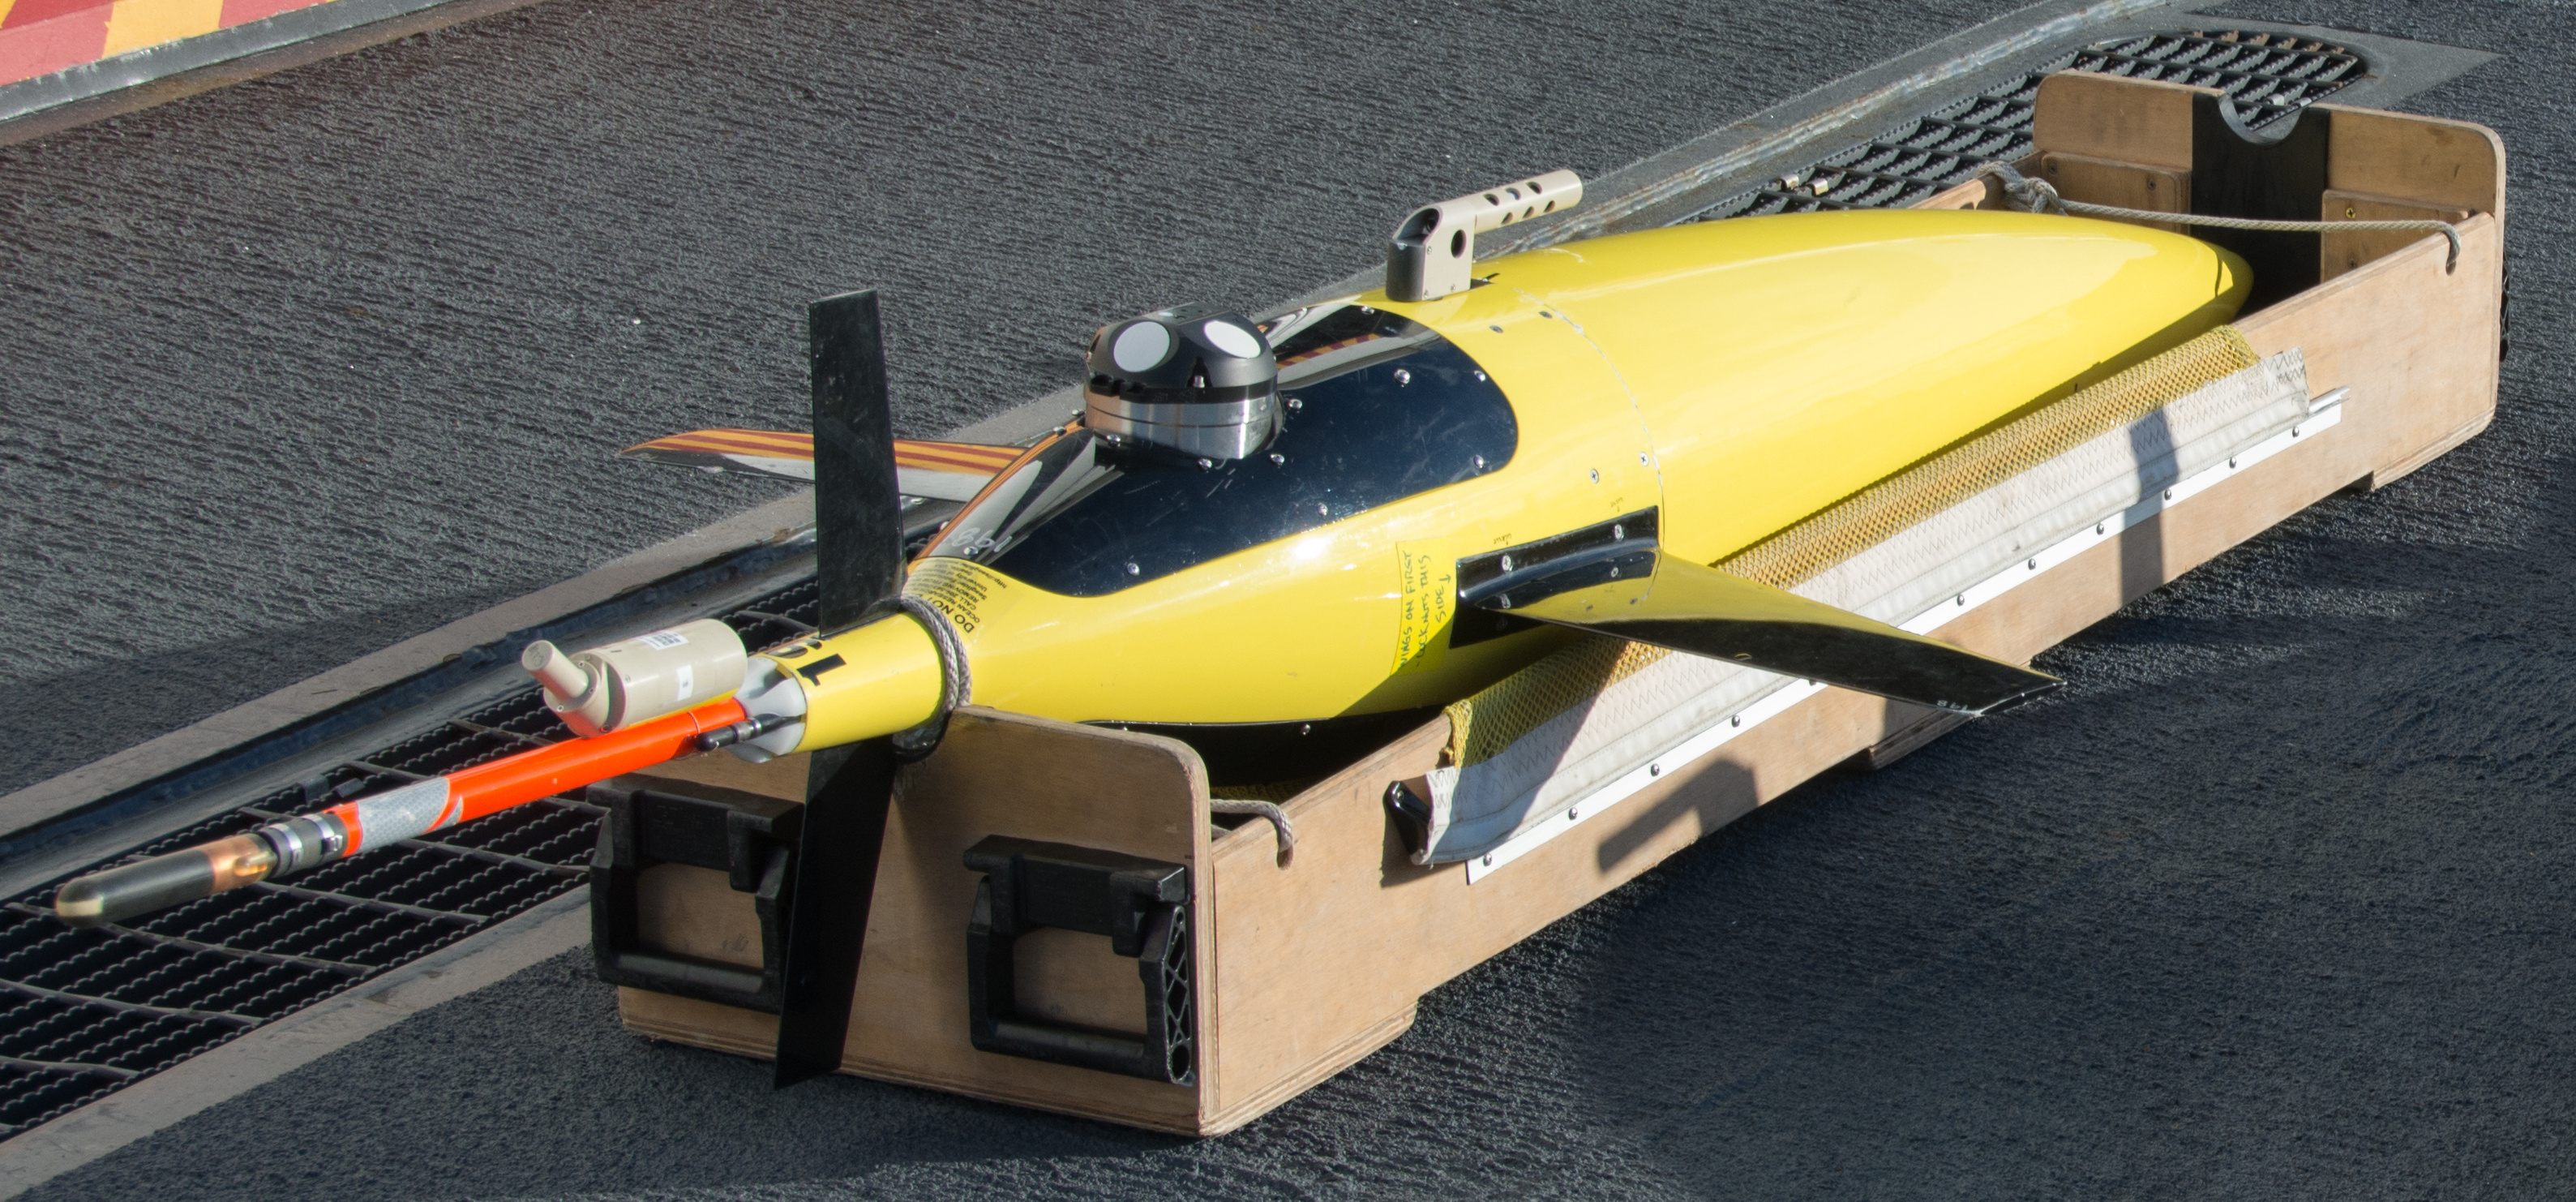
\includegraphics[width=3.0in]{./figs/Gliders_hires-99_crop.jpg}
  %\vspace{-0.1in}
  \caption{Seaglider AUG with an upwards-facing ADCP installed in aft fairing.}
  \label{fig.SG}
%   \vspace{-0.1in}
  %\rule{\textwidth}{0.02in}
  \vspace{-0.2in}
\end{figure}

The main challenge of AUG-based ADCP velocity profiling is that each velocity profile is measured relative to the TTW motion of the glider, which is generally unknown. TTW velocity can be inferred from the AUG dynamic model, but is subject to uncertainty because the model is based on steady state flight and doesn't take roll into account. This lack of a georeferenced platform velocity produces the need to perform a simultaneous robust estimation of current and glider TTW velocity using all available data -- ADCP velocity profiles, surrounding water density, glider buoyancy engine state, glider attitude and angle of attack, glider depth, and GPS positions at the start and end of the dive. Figure 2 shows a short section of the dive with the individual ADCP profiles, offset by our initial estimate of the AUG's TTW velocity (i.e., the velocity from the hydrodynamic model, without accounting for current-induced motion). The thick black line is the estimated current profile. This is from a 750 m dive, so the sections of data shown were collected 3.5 hrs apart. The difference in the current profile during ascent and descent are clearly visible, motivating the need for different current profiles during ascent and descent.

\begin{figure}[!ht]
  \centering
  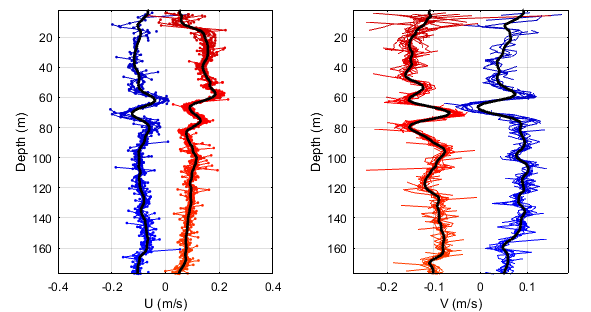
\includegraphics[width=\columnwidth]{./figs/current_profile_snip.png}
  \vspace{-0.1in}
  \caption{ Overlapped ADCP profiles during descent (blue) and ascent (red) for dive 116 of sg198. The fitted current profile is shown as the thick black line.}
  \label{fig.profile_snip}
   \vspace{-0.1in}
  %\rule{\textwidth}{0.02in}
%   \vspace{-0.2in}
\end{figure}

\begin{thebibliography}{1}

\bibitem{Todd2017}
Todd, R.E., D.L. Rudnick, J.T. Sherman, W.B. Owens, L. George, Absolute velocity estimates from autonomous underwater gliders equipped with Doppler current profilers, \emph{J. Atmos. Oceanic Technol.}, 34(2), 309–333.%, doi:10.1175/JTECH-D-16-0156.1.

\bibitem{Todd2011}
Todd, R.E., D.L. Rudnick, M.R. Mazloff, R.E. Davis, B.D. Cornuelle, Poleward flows in the southern California Current System: Glider observations and numerical simulation, \emph{J. Geophys. Res.}, 116, C02026. %, doi:10.1029/2010JC006536.

\end{thebibliography}

\begin{abstract}
    
This paper describes the development and experimental results of navigation algorithms for an autonomous underwater glider (AUG) that employs an on-board acoustic Doppler current profiler (ADCP). AUGs are buoyancy-driven autonomous underwater vehicles that use small hydrofoils to make forward progress while profiling vertically.
%
During each dive, which can last up to 6 hours, the Seaglider AUG used in this experiment typically reaches the depth of 1000 m and travels 3-6 km horizontally through the water, relying solely on dead-reckoning. Horizontal through-the-water (TTW) progress of AUG is 20-30 cm/s, which is comparable to the speed of the stronger ocean currents. Underwater navigation of an AUG in the presence of unknown advection therefore presents a considerable challenge. We present a post-processing algorithm to simultaneously estimate the ocean current profile through which the AUG was flown, as well as the AUG's horizontal position as influenced by the local currents. 
%
Results are demonstrated using 1 MHz ADCP data collected from two Seaglider AUGs deployed for 49 days off the north coast of Alaska during August and September 2017. ... say soemthing quantitative if possible ...

\end{abstract}


% TO DO
% Add Lora as an author
% 
%

\section{Introduction}

The goal of this work is to simultaneously estimate a) absolute (Earth-referenced) ocean velocity profile, and b) the absolute autonomous underwater glider (AUG) path over the bottom, based on on-board acoustic Doppler current profiler (ADCP) observations of relative current velocity profiles. 

The main challenge of AUG-based ADCP velocity profiling is that each velocity profile is measured relative to the through-the-water (TTW) motion of the glider, as opposed to the earth referenced glider velocity. The AUG's TTW velocity can be inferred from the AUG dynamic model, but is subject to uncertainty because the model is based on steady state flight and doesn't take roll into account. This lack of a georeferenced platform velocity produces the need to perform a simultaneous robust estimation of current and glider TTW velocity using all available data -- ADCP velocity profiles, surrounding water density, glider buoyancy engine state, glider attitude and angle of attack, glider depth, and GPS positions at the start and end of the dive.

In this paper we will describe two different frameworks for performing this estimation. A linear global inverse, and a fast, robust nonlinear method. For comparison purposes in this initial work, we will use a pre-computed estimate of the glider TTW velocity from the hydrodynamic model for both methods. The goal, however, is to also incorporate the nonlinear hydrodynamic model estimation as part of the nonlinear estimation framework. We will also investigate the effect of including either a subsea position fix from range measurements during a small portion of the glider's flight.

\section{Background}

%Extensive work by Todd et al in this domain employed a modified version of the lowered ADCP estimation framework \cite{todd-2017-JAOT,todd-2011-JGRC}.  In addition to this estimation framework, our work uses current data from the entire dive (as opposed to just during descent) and incorporates nonlinear hydrodynamic and attitude models from the vehicle navigation system to produce a time-varying current profile for the entire dive.

Historically, ADCP measurements were made from ships with with relatively low frequency systems (70 kHz) or from moorings with low or mid-frequency instruments (300 kHz). The 300 kHz ADCPs are also common on large underwater vehicles, in particular instruments that can be used as a Doppler velocity log to provide ``bottom lock''---i.e., vehicle velocity relative to the seafloor \cite{yoerger-1998-ABE} or, in some specialized cases, the underside of ice \cite{mcfarland-2015-icerelnav}.

To provide better resolution of deep currents from shipboard measurements, lowered ADCP methods were developed using overlapping shear traces from a higher frequency (300 kHz) ADCP lowered from a (relatively) stationary ship. The shear traces are then used to reconstruct the full current profile \cite{Visbeck2002}.

In the last 10 years, there has been increased interest in using ADCPs from autonomous underwater vehicles to characterize the currents between the surface and the seafloor and to close the gap of uncertainty in vehicle drift between when GPS is available at the surface and bottom lock is obtained within range of the seafloor \cite{mstanway-2010a,medagoda10_oceans}.

Even more recently, very high frequency ADCPs (1 MHz) have been integrated onto underwater autonomous gliders---initially the Slocum gliders, and now onto Seagliders---and used to estimate depth-varying current profiles. 

\emph{ANDREY -- I think this is the reference we are missing \cite{thurnherr-2015-slocum-adcp}. \\
https://ieeexplore.ieee.org/document/7098134 \\
%https://ieeexplore.ieee.org/document/7098134
Can you summarize how it compares to your method? I admit the reviewer's comment sure sound like it could have been from Lou St. Laurent!}

Extensive work by Todd et al in this domain employed a modified version of the lowered ADCP estimation framework \cite{todd-2011-JGRC,todd-2017-JAOT}.
%
Our contribution builds on and extends their work with several key innovations. We use current data from the entire dive (as opposed to just during descent), which is crucial for multi-hour dives where, as we show, the current profiles on descent versus ascent differ significantly. We also separate the over-the-ground glider velocity into the drift velocity (as a result of advection), and the glider's horizontal through-the-water velocity. This enables us to directly incorporate hydrodynamic model velocity estimates and independently control the smoothness regularization of the different velocity components.
\section{Linear Method \textbf(ANDREY)}

Andrey's method

Is this the right title?



\section{Current and State-Space Deconvolution via Extended Smoothing}
\label{sec:nonlin}



\section{Experimental Data Collection}
 
%Each glider was equipped with a Nortek Signature1000 1 MHz ADCP. Figure \ref{fig.SG} shows an ADCP installed, facing upwards, in the tail section of one of the AUGs. The ADCPs are configured by Nortek to use only three beams---in the upward-facing position, those are the two side beams and the aft beam during descent, and the two side beams and the forward beam during ascent. The ADCPs were programmed to collect a profile every 15 seconds. Each profile covers up to 20 m depth, with a new profile starting approximately every 1.5 m (i.e., the vertical distance covered by the AUG in 15 seconds).
 
 As part of the Canada Basin Glider Experiment (CABAGE), two Seagliders, SG196 and SG198, were deployed on 6 August 2017 at the shelf break north of Prudhoe Bay, AK. From there, they flew up to and around the CANAPE mooring array until they were recovered on 17 September 2017, for a total of 49 days.  Together the gliders covered approximately 1730 km over the course of 712 dives, with SG196 diving to 480 m depth and SG198 diving to 750 m.  Figure \ref{fig:track} shows the glider tracklines for both a short test deployment in 2016 and the 2017 deployment.

\begin{figure}%[!ht]
  \centering
  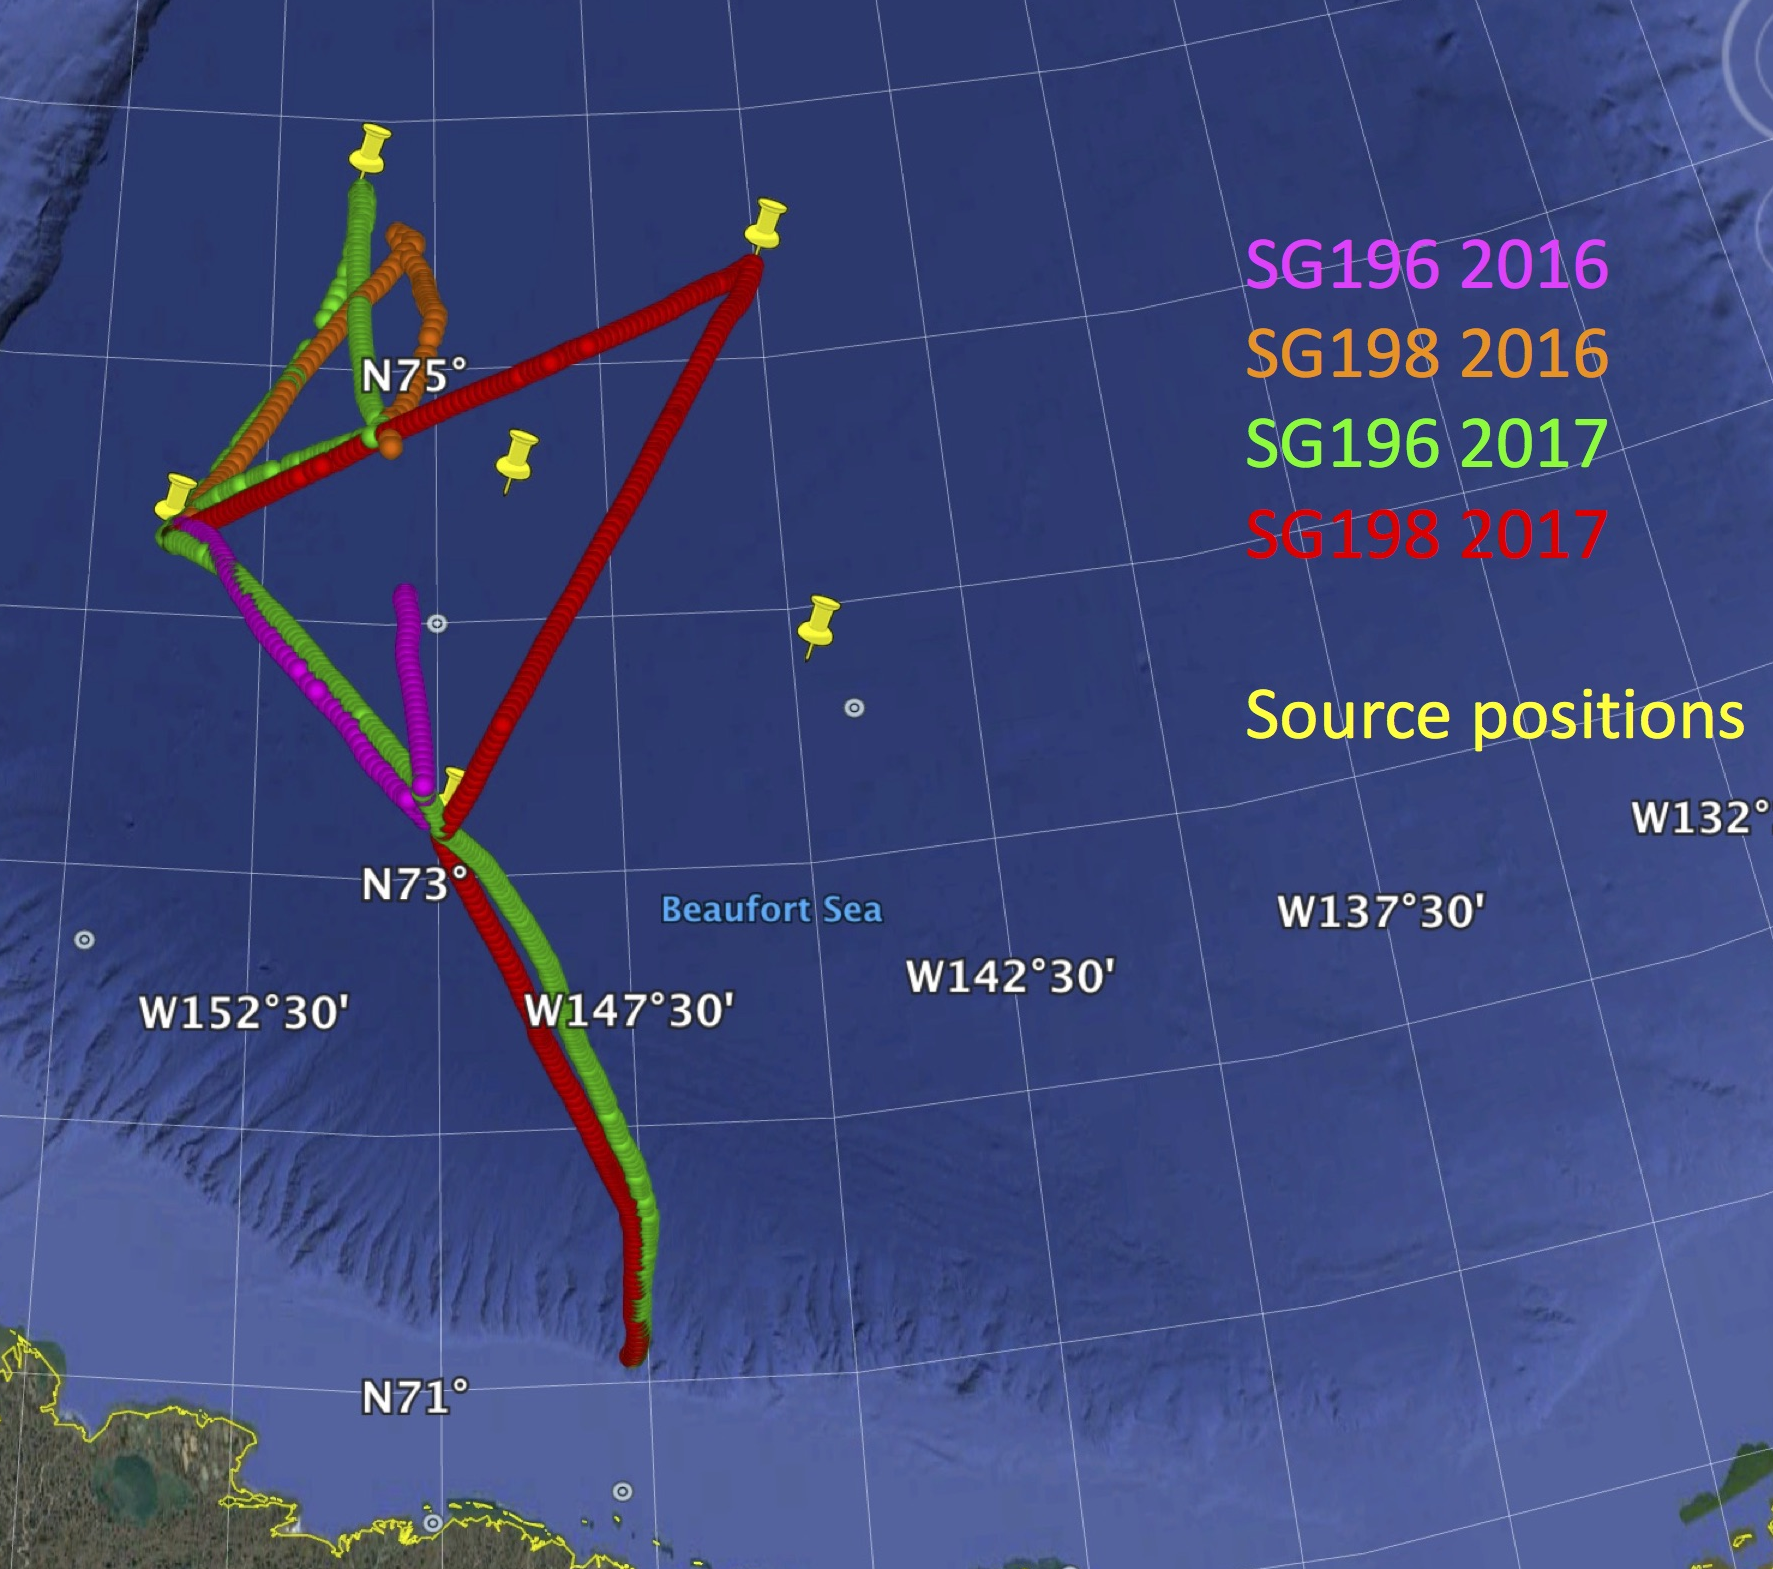
\includegraphics[width=0.9\columnwidth]{./figs/GliderTrajCombined.png}%{./figs/CABAGE_sg198_track_quicklook.png}
  \caption{SG196 and SG198 were deployed at the shelf break north of Prudhoe Bay, AK.  From there, they flew up to and around the CANAPE mooring array until, 49 days later, they were recovered by the USCGC Healy.}
  \label{fig:track}
\end{figure}

Each glider was equipped with a Nortek Signature1000 1 MHz ADCP, as well as the standard suite of conductivity temperature (CT) sensor, pressure sensor, WHOI MicroModem, and custom-built passive marine acoustic recorders (PMARs). Figure \ref{fig:SG} shows the gliders loaded on the R/V Ukpik, ready for launch, with the upward-facing ADCPs, installed in the tail section, clearly visible.

\begin{figure}%[!ht]
  \centering
%  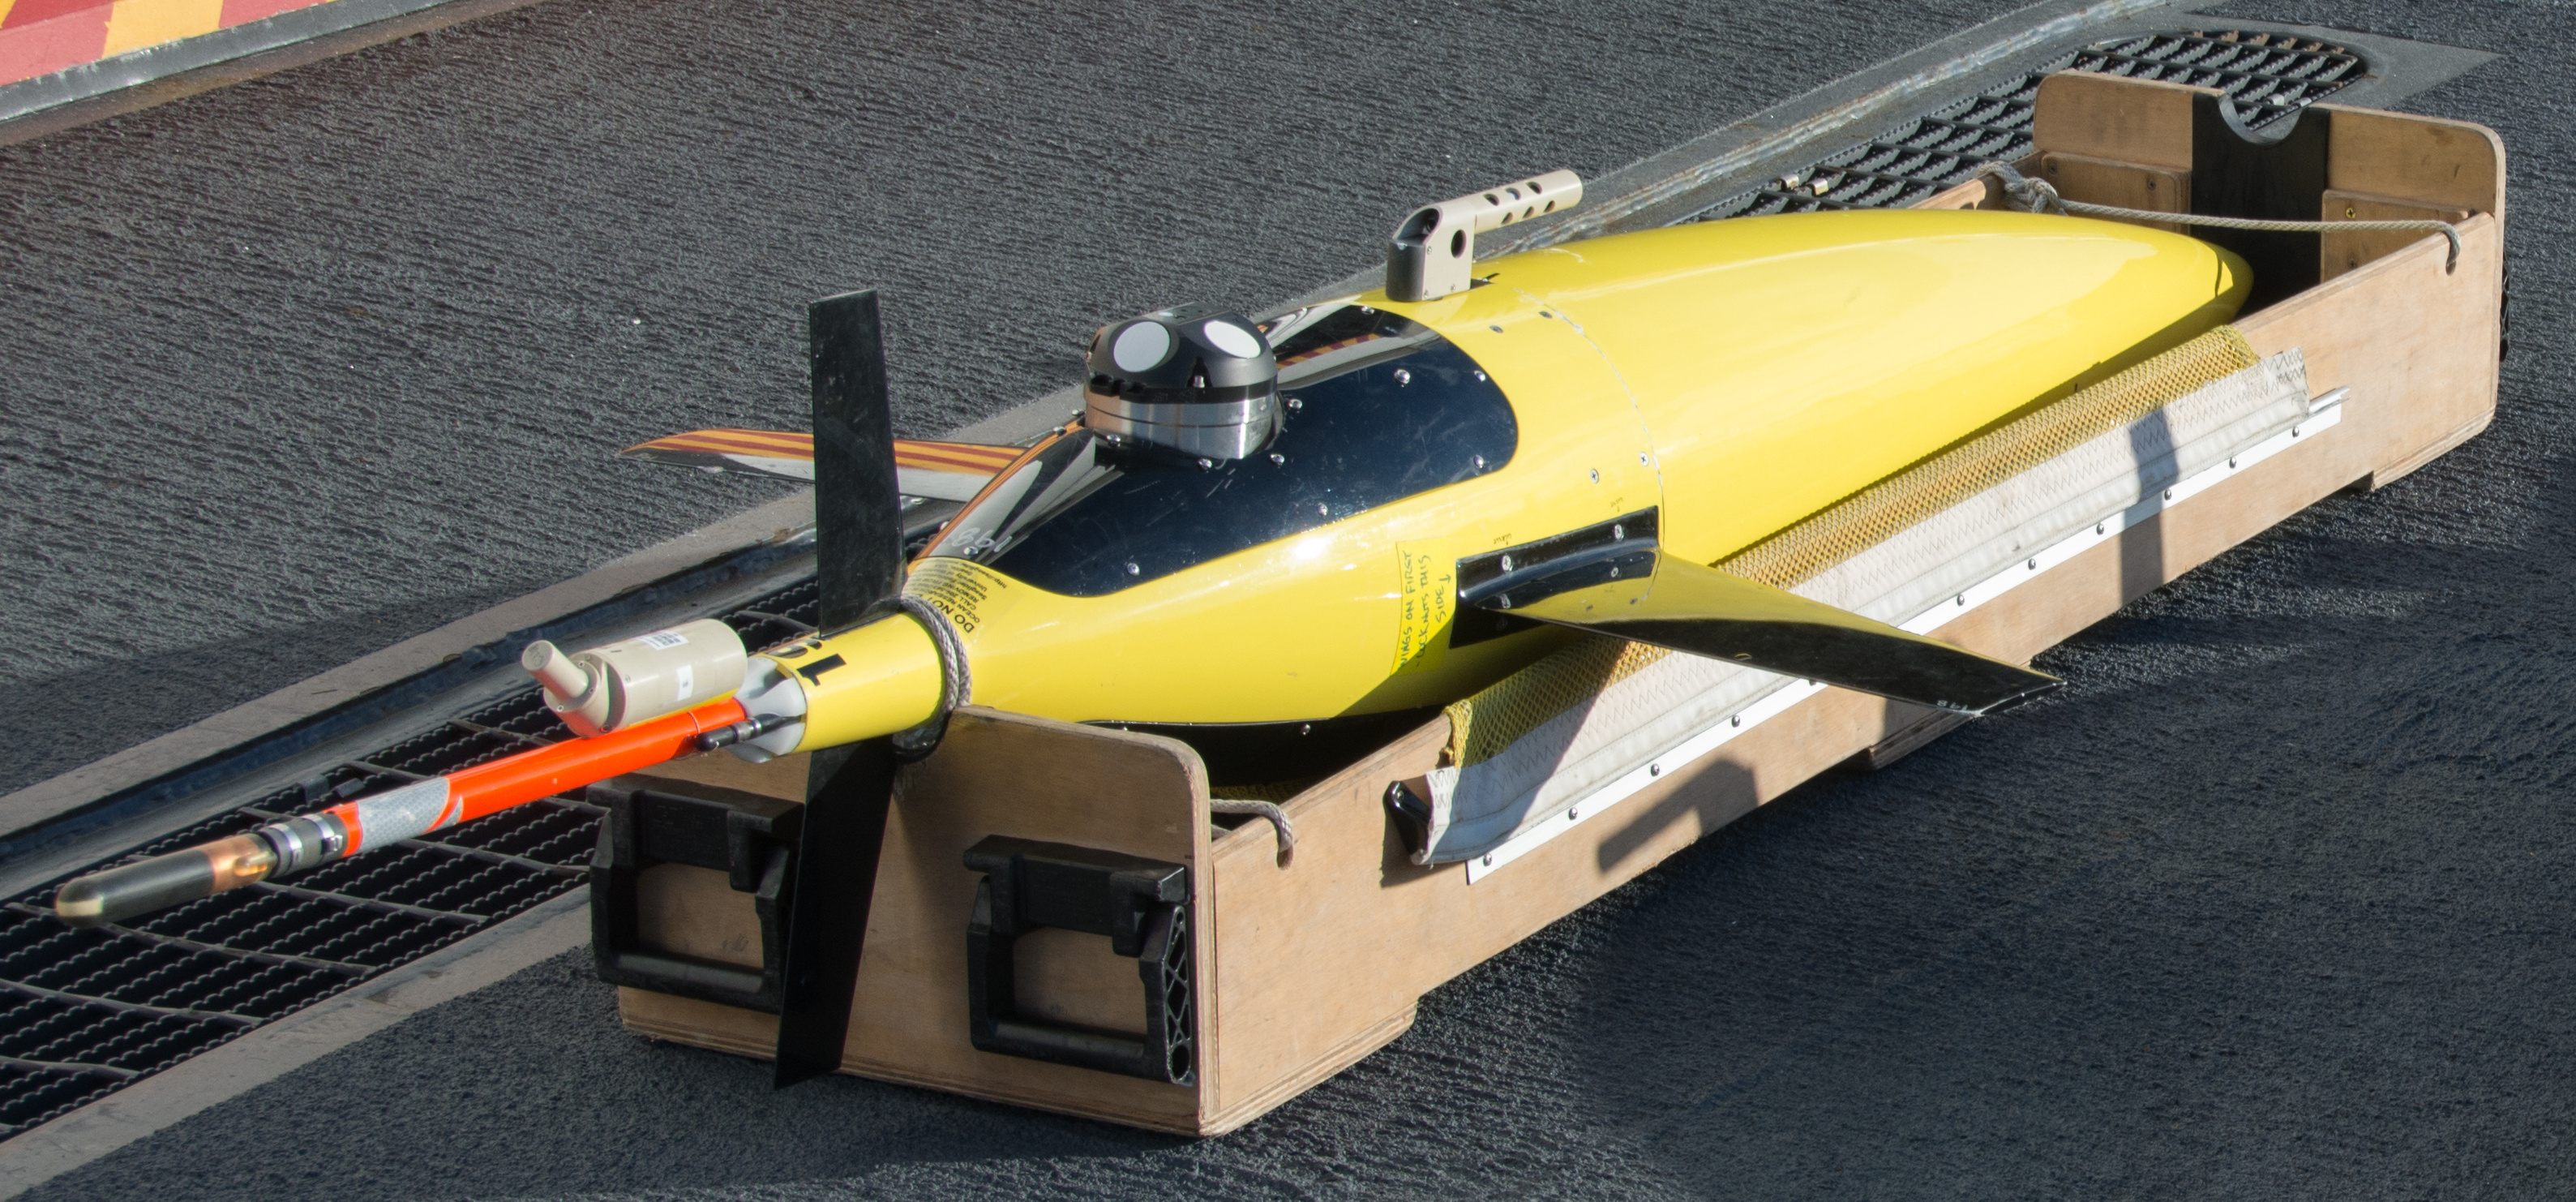
\includegraphics[width=0.6\columnwidth]{./figs/Gliders_hires-99_crop.jpg}
%  \vspace{0.2cm}
  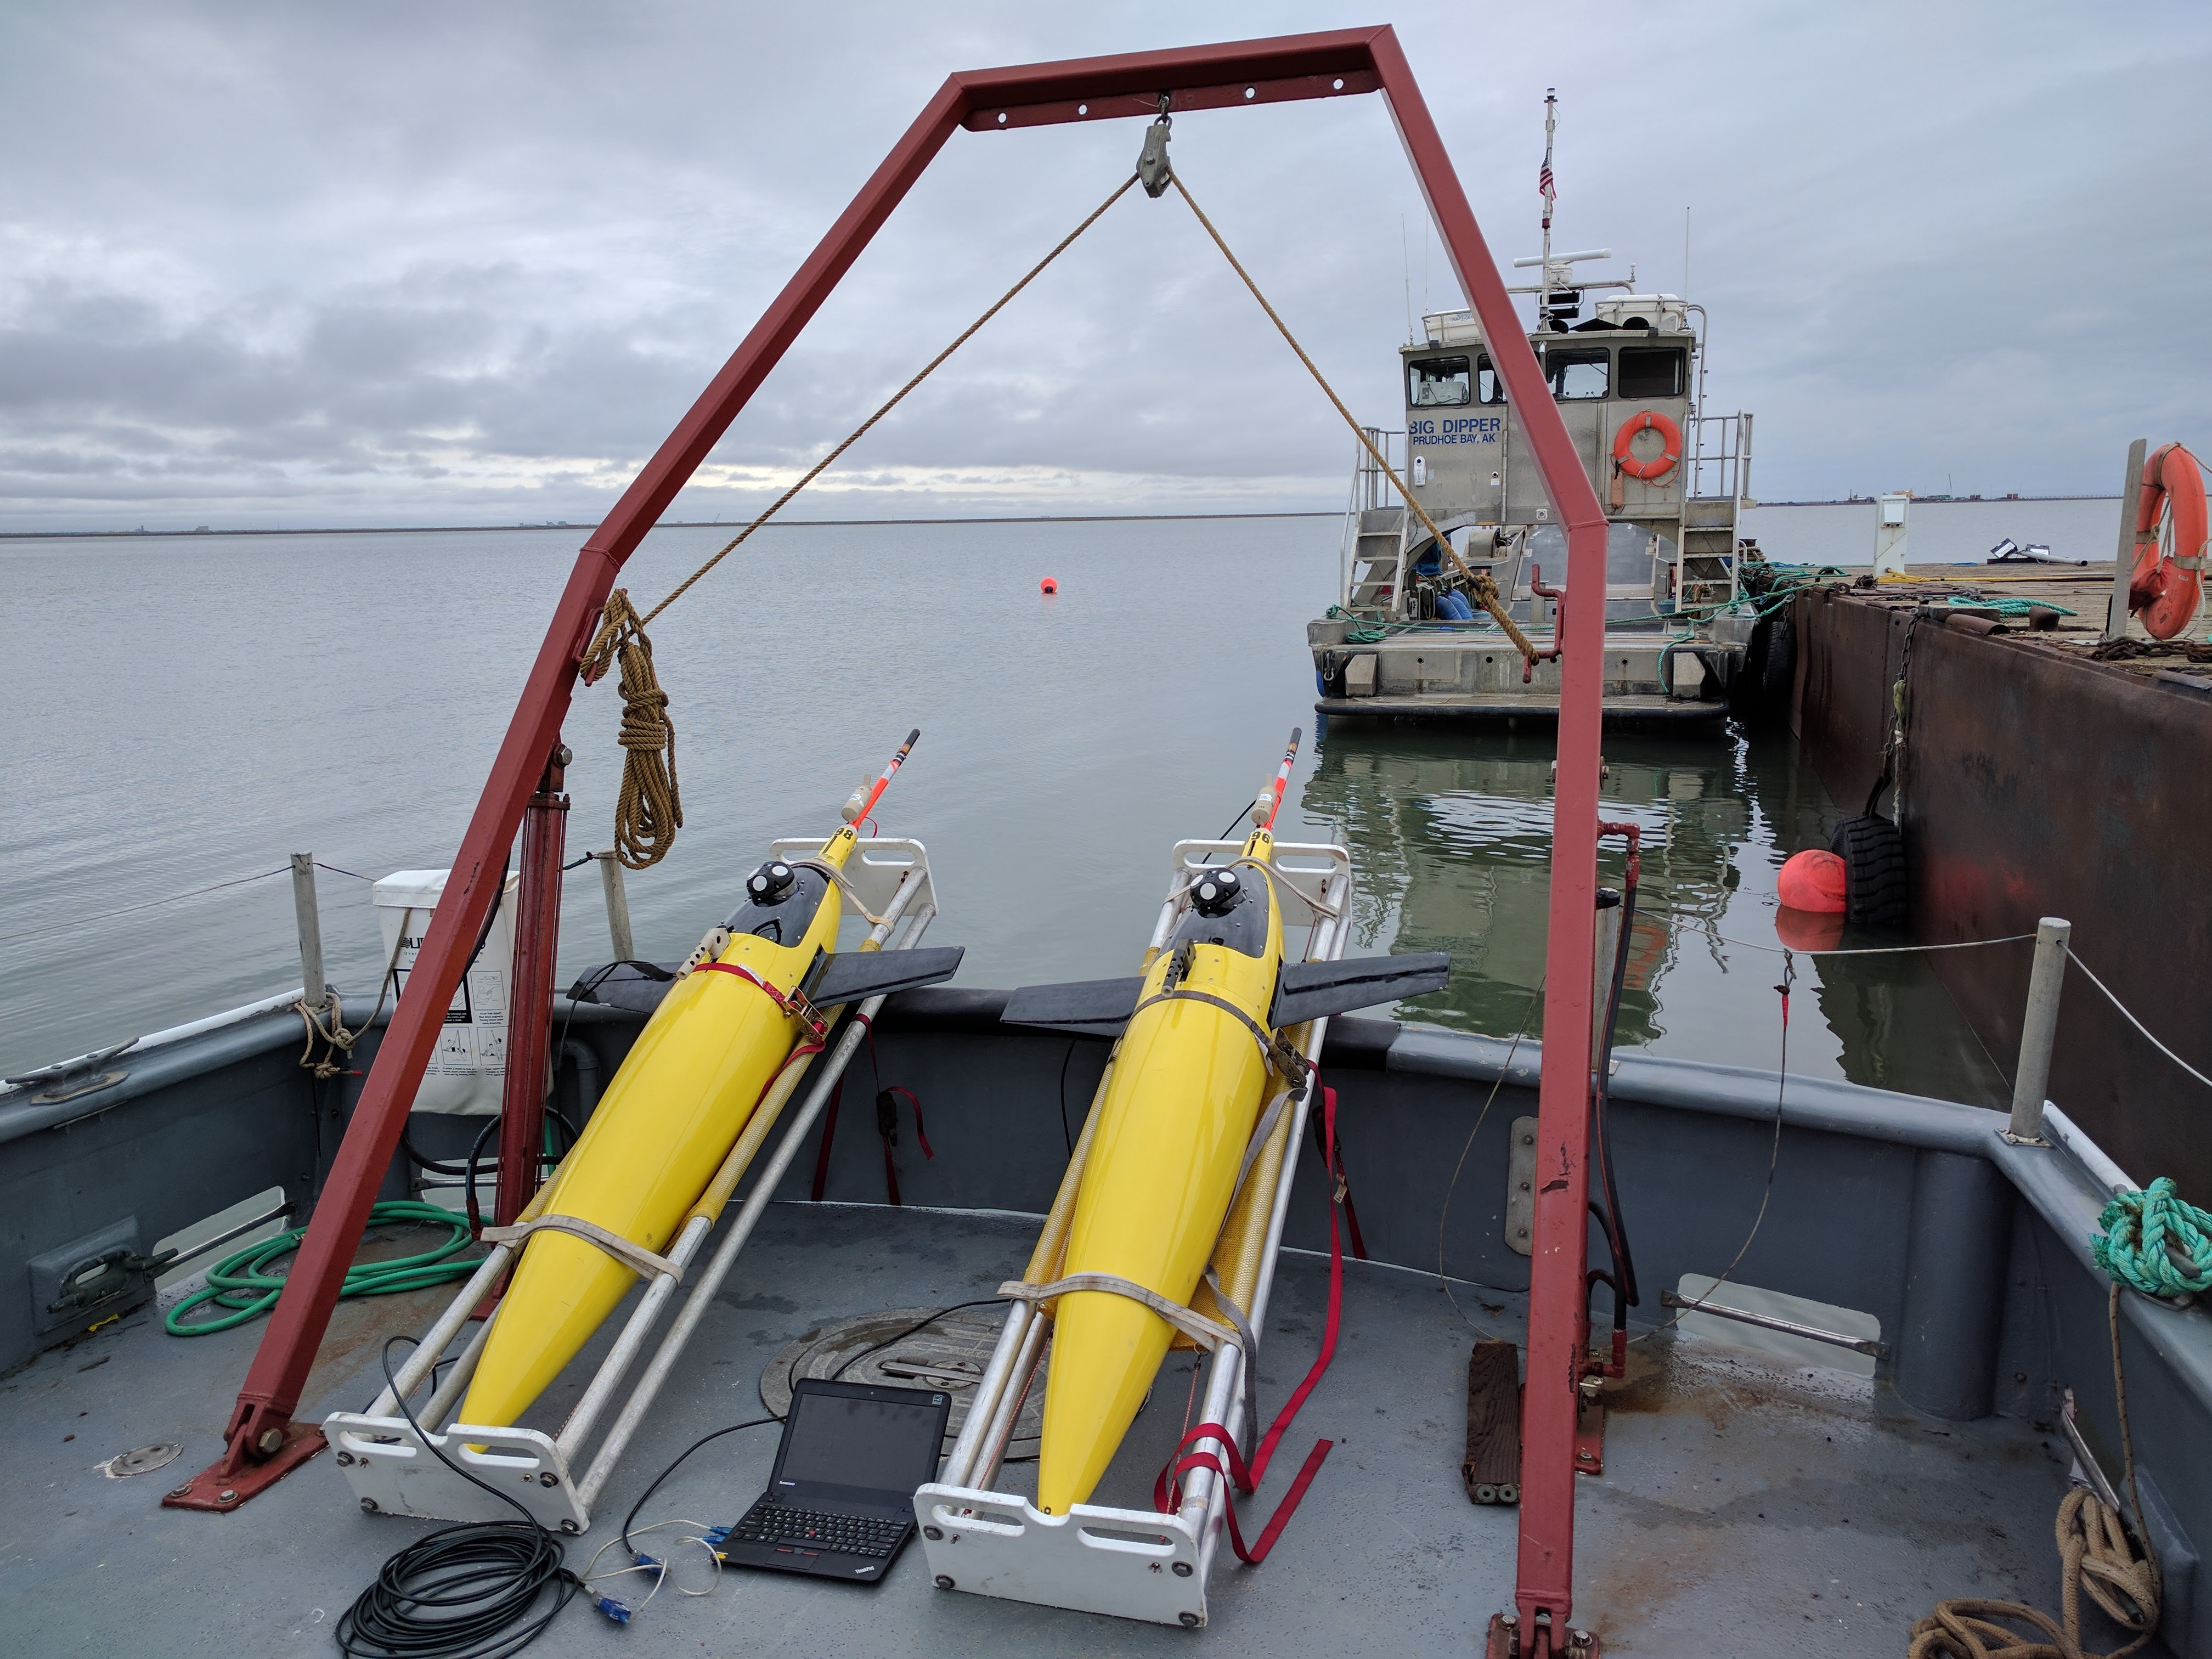
\includegraphics[width=0.9\columnwidth]{./figs/UkpikGliders.jpg}
  \caption{Ready for launch, SG196 and SG198 are loaded on the R/V Ukpik in Prudhoe Bay, AK, with the upward-facing ADCPs, installed in the aft fairing, clearly visible. }
  \label{fig:SG}
  \vspace{-0.2in}
\end{figure}

\begin{figure}%[!ht]
  \centering
  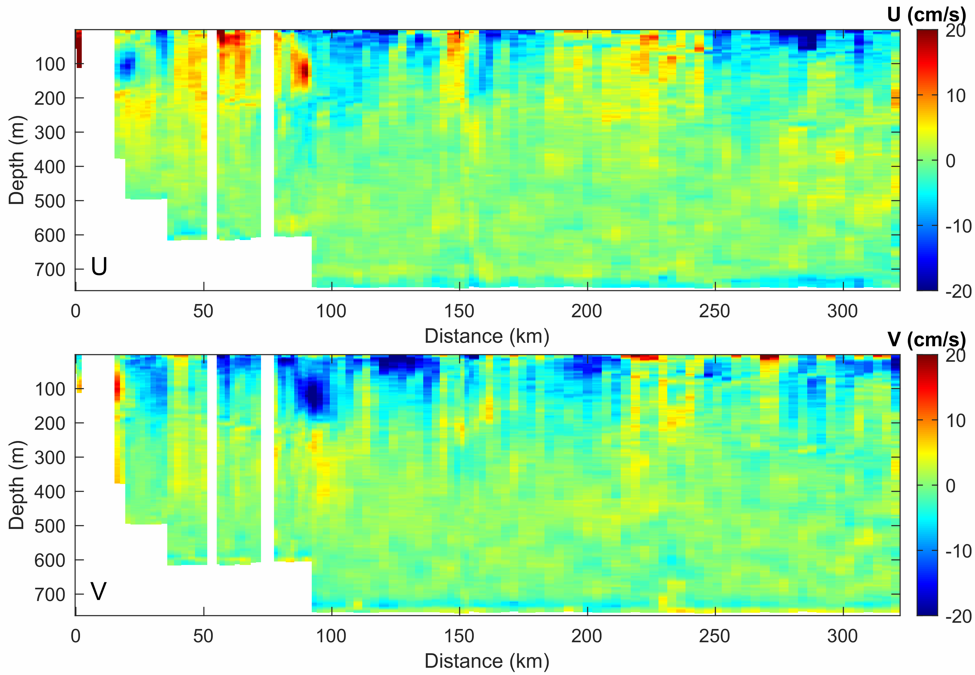
\includegraphics[width=0.9\columnwidth]{./figs/CABAGE_sg198_ADCP_quicklook.png}
  \caption{An example of the cumulative ADCP data collected by SG198 during the first few hundred kilometers of the deployment.}
  \label{fig:ADCP}
\end{figure}

For clarity during the discussion here, when referring to the ADCP data, we will use \emph{trace} to refer to an individual profile collected by the ADCP, and \emph{profile} to refer to the result of the inverse, i.e. the current profile for the entire dive. The ADCPs were programmed to collect a trace every 15 seconds with 2.0 m bins. Each trace typically covered 25m depth, with the actual usable range varying with the amount of acoustic scatterers in the water. As a result, with the typical vertical descent rate of 10 cm/s, any
given depth bin was covered by 15-16 different traces.  Figure \ref{fig:ADCP} illustrates the cumulative ADCP data collected by SG198 during the first few hundred kilometers of the 49-day deployment.
 
%\begin{figure}[!ht]
%  \centering
%  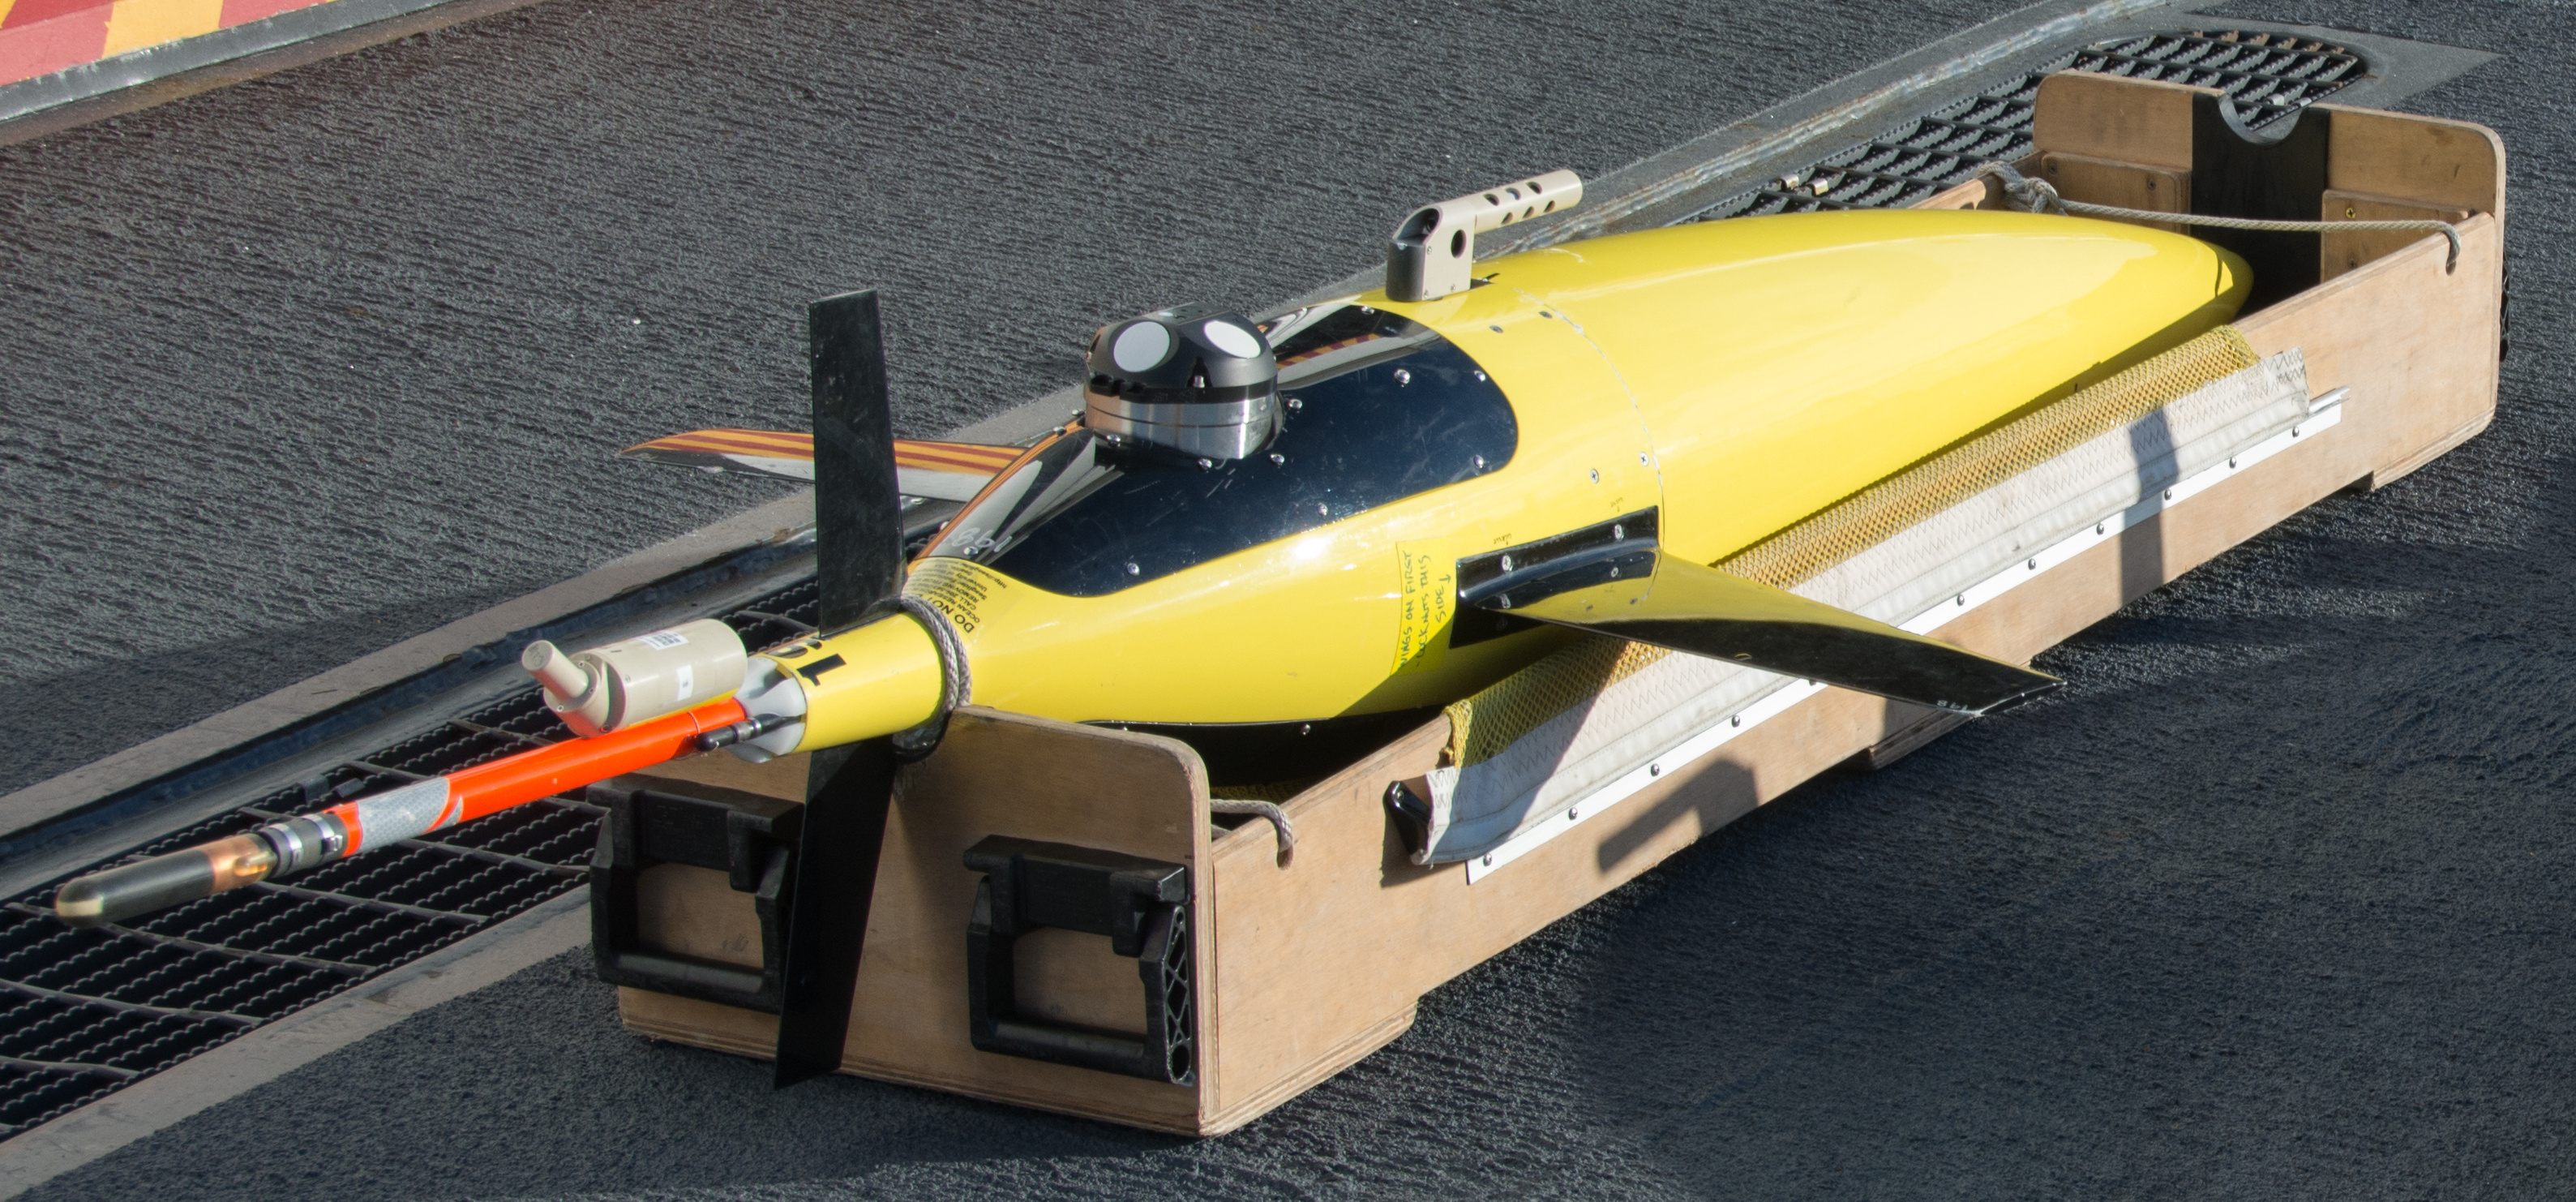
\includegraphics[width=3.0in]{./figs/Gliders_hires-99_crop.jpg}
%  %\vspace{-0.1in}
%  \caption{Seaglider AUG with an upwards-facing ADCP installed in aft %fairing.}
%  \label{fig.SG}
%%   \vspace{-0.1in}
%  %\rule{\textwidth}{0.02in}
%  \vspace{-0.2in}
%\end{figure}

\section{Results}

 for several cases:
- not trusting/using  the EKF velocities
- trusting the EKF velocities
- using a single subsea position fix or multiple subsea range measurements to further constrain the output (I think only the nonlinear model can do this gracefully / easily?)
And then using ground truth from one of the mooring for comparison.

\begin{figure}%[!ht]
%  \centering
%  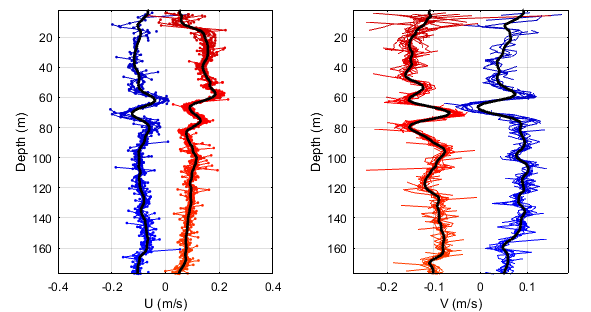
\includegraphics[width=\columnwidth]{./figs/current_profile_snip.png}
  \vspace{1.5in}
  \caption{The above plot shows a comparison of the results from the linear method with and without knowledge of the glider's through-the-water (TTW) velocity. On the left hand side is a snippet of the aligned individual traces and the resulting current estimate. On the right hand side is the resulting glider trajectory of a single candidate dive, in this case, dive \# XXX. The top plots show results produced without knowledge of the glider's TTW velocity (blue line), where the difference between overlapping traces is minimized while producing a current profile such that the glider ends up at the end-of-dive GPS. The lower plots show results produced when including knowledge of the glider's TTW velocity, in this case with a weighting of 0.8 (black line). This produces a more sensical glider trajectory in that...}
  \label{fig.linear}
\end{figure}


\begin{figure}%[!ht]
%  \centering
%  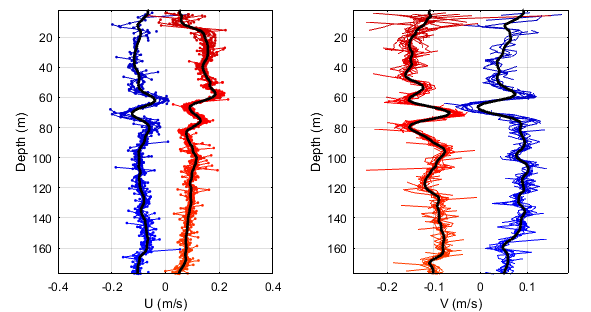
\includegraphics[width=\columnwidth]{./figs/current_profile_snip.png}
  \vspace{1.5in}
  \caption{The above plot shows a similar comparison as Figure \ref{fig.linear}, but for the nonlinear method...}
  \label{fig.nonlinear}
\end{figure}

\begin{figure}%[!ht]
%  \centering
%  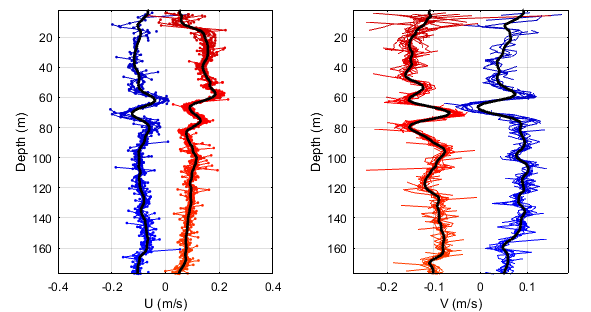
\includegraphics[width=\columnwidth]{./figs/current_profile_snip.png}
  \vspace{1.5in}
  \caption{The above plot shows a comparison between the the linear, nonlinear, and ground truth as obtained from a 300 kHz ADCP on the T4 mooring...}
  \label{fig.mooring}
\end{figure}


\begin{figure}%[!ht]
%  \centering
%  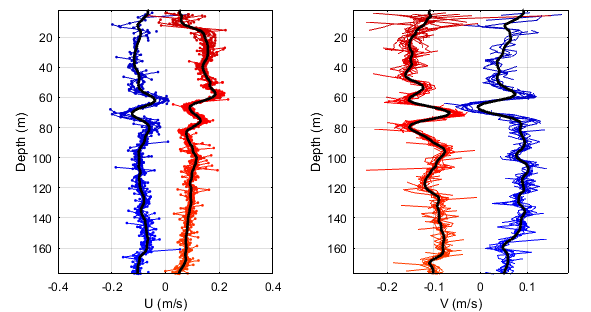
\includegraphics[width=\columnwidth]{./figs/current_profile_snip.png}
  \vspace{1.5in}
  \caption{The above plot shows the results from the nonlinear method, this time incorporating an additional subsea fix, arred at using 4 range measurements received over 37 minutes while the AUG was decending from 3042m and 581m. On the left is the current profile, compared to the ground truth from the mooring. On the right is the glider trajectory.}
  \label{fig.subseafix}
\end{figure}


% Figure \ref{fig.profile_snip} shows a short section of the dive with the individual ADCP profiles, offset by our initial estimate of the AUG's TTW velocity (i.e., the velocity from the hydrodynamic model, without accounting for current-induced motion). The thick black line is the estimated current profile. This is from a 750 m dive, so the sections of data shown were collected 3.5 hrs apart. The difference in the current profile during ascent and descent are clearly visible, motivating the need for different current profiles during ascent and descent.

% \begin{figure}[!ht]
%   \centering
%   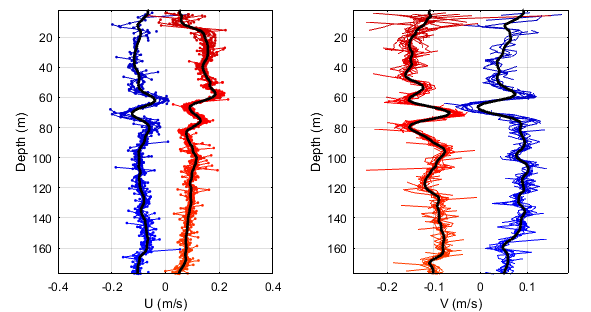
\includegraphics[width=\columnwidth]{./figs/current_profile_snip.png}
%   \vspace{-0.1in}
%   \caption{ Overlapped ADCP profiles during descent (blue) and ascent (red) for dive 116 of sg198. The fitted current profile is shown as the thick black line.}
%   \label{fig.profile_snip}
%   \vspace{-0.1in}
%   %\rule{\textwidth}{0.02in}
% %   \vspace{-0.2in}
% \end{figure}


\section{Conclusions and Future Work \textbf(SARAH)}


\section*{Acknowledgements \textbf(SARAH)}
We would like to acknowledge...


\bibliographystyle{IEEEtran}
\bibliography{sew_additional}

% that's all folks
\end{document}